\documentclass[10pt,twocolumn,fleqn]{IEEEtran}

%% set page size to US letter
\special{papersize=8.5in,11in}
\setlength{\pdfpageheight}{\paperheight}
\setlength{\pdfpagewidth}{\paperwidth}

\DeclareMathAlphabet{\mathtsl}{OT1}{ptm}{m}{sl}
\RequirePackage{amssymb}
\usepackage{hyperref}
\usepackage{xspace}
\usepackage{algorithm}
\usepackage[noend]{algpseudocode}
\usepackage{amsbsy}
\usepackage{amsthm}
\usepackage{graphicx}
\usepackage{helvet}
\usepackage{enumerate}
\usepackage{amsmath}
\usepackage{amstext}
\usepackage{amsfonts}
\usepackage{graphicx}
\usepackage{multirow}
\usepackage{subfig}
\usepackage{comment}
\usepackage{cases}
\usepackage{xcolor}
\usepackage{epstopdf}
\usepackage[normalem]{ulem}
\usepackage{diagbox}
% \usepackage{titlesec}
% \titlespacing*{\section}{0pt}{1.1\baselineskip}{\baselineskip}

% \newcommand{\B}{{\mathbb{B}}}
\newcommand{\Z}{{\mathbb{Z}}}
\newcommand{\R}{{\mathbb{R}}}
\newcommand{\Q}{{\mathbb{Q}}}
\newcommand{\N}{{\mathbb{N}}}
\newcommand{\C}{{\mathbb{C}}}
\newcommand{\Zn}{{\mathbb{Z}}_{n}}
\newcommand{\Zp}{{\mathbb{Z}}_{p}}
\newcommand{\F}{{\mathbb{F}}}
\newcommand{\FF}{{\mathcal{F}}}
\newcommand{\Fbar}{{\overline{\mathbb{F}}}}
\newcommand{\Fq}{{\mathbb{F}}_{q}}
\newcommand{\Fqbar}{{\overline{{\mathbb{F}}_q}}}
\newcommand{\Fkk}{{\mathbb{F}}_{2^k}}
\newcommand{\Zkk}{{\mathbb{Z}}_{2^k}}
\newcommand{\Fkkx}[1][x]{\ensuremath{\mathbb{F}}_{2^k}[#1]\xspace}
\newcommand{\Grobner}{Gr\"{o}bner\xspace}
\newcommand{\bi}{\begin{itemize}}
\newcommand{\ei}{\end{itemize}}

\newcommand{\idealj}{{J = \langle f_1, \dots, f_s\rangle}}
\newcommand{\idealg}{{J = \langle g_1, \dots, g_t\rangle}}
\newcommand{\vfqj}{{V_{\Fq}(J)}}
\newcommand{\vfkkj}{{V_{\Fkk}(J)}}

%%% Added by Utkarsh %%%
\newcommand{\Va}{{V_A}}
\newcommand{\Vb}{{V_B}}
\newcommand{\Vc}{{V_C}}
\newcommand{\Vbc}{{V_{B,C}}}
\newcommand{\Vabc}{{V_{A,B,C}}}
\newcommand{\Vac}{{V_{A,C}}}
\newcommand{\w}{\wedge}

%%%%%%%%%%%%%%%%%%%%%%%%

\newcommand{\blu}{\color{blue}}
% \newcommand{\Grobner}{Gr\"{o}bner\xspace}
\newcommand{\fqring}{\Fq[x_1,\dots,x_n]}


% New command for the line spacing.
\newcommand{\ls}[1]
    {\dimen0=\fontdimen6\the\font
     \lineskip=#1\dimen0
     \advance\lineskip.5\fontdimen5\the\font
     \advance\lineskip-\dimen0
     \lineskiplimit=.9\lineskip
     \baselineskip=\lineskip
     \advance\baselineskip\dimen0
     \normallineskip\lineskip
     \normallineskiplimit\lineskiplimit
     \normalbaselineskip\baselineskip
     \ignorespaces
    }
% New command for the table bnotes.
\def\tabnote#1{{\small{#1}}}

\newcommand{\beqarr}{\begin{eqnarray}}
\newcommand{\eeqarr}{\end{eqnarray}}
\newcommand{\ov}{\bar}
\newcommand{\xor}{\bigoplus}
\newcommand{\Fm}{{\mathbb{F}}}
\newcommand{\myfontsize}{\fontsize{7}{9}\selectfont}
\newcommand{\Ftwo}{{\mathbb{F}}_{2}}
\newcommand{\G}{{\mathcal{G}}}
\newcommand{\alert}[1]{\textcolor{red}{#1}}
\newcommand{\B}{{\mathbb{B}}}
\newcommand{\Z}{{\mathbb{Z}}}
\newcommand{\R}{{\mathbb{R}}}
\newcommand{\Q}{{\mathbb{Q}}}
\newcommand{\N}{{\mathbb{N}}}
\newcommand{\C}{{\mathbb{C}}}
\newcommand{\Zn}{{\mathbb{Z}}_{n}}
\newcommand{\Zp}{{\mathbb{Z}}_{p}}
\newcommand{\F}{{\mathbb{F}}}
\newcommand{\FF}{{\mathcal{F}}}
\newcommand{\Fbar}{{\overline{\mathbb{F}}}}
\newcommand{\Fq}{{\mathbb{F}}_{q}}
\newcommand{\Fqbar}{{\overline{{\mathbb{F}}_q}}}
\newcommand{\Fkk}{{\mathbb{F}}_{2^k}}
\newcommand{\Zkk}{{\mathbb{Z}}_{2^k}}
\newcommand{\Fkkx}[1][x]{\ensuremath{\mathbb{F}}_{2^k}[#1]\xspace}
\newcommand{\Grobner}{Gr\"{o}bner\xspace}
\newcommand{\bi}{\begin{itemize}}
\newcommand{\ei}{\end{itemize}}
\newcommand{\idealj}{{J = \langle f_1, \dots, f_s\rangle}}
\newcommand{\idealf}{{F = \{f_1, \dots, f_s\}}}
\newcommand{\idealg}{{J = \langle g_1, \dots, g_t\rangle}}
\newcommand{\vfqj}{{V_{\Fq}(J)}}
\newcommand{\vfkkj}{{V_{\Fkk}(J)}}
\newcommand{\vfqjo}{{V_{\Fq}(J_0)}}
\newcommand{\vfbqj}{{V_{\overline{\Fq}}(J)}}
\newcommand{\vfbqjo}{{V_{\overline{\Fq}}(J_0)}}
\newcommand{\vfbqjjo}{{V_{\overline{\Fq}}(J+J_0)}}
\newcommand{\acf}{\bar{F}_q}
\newcommand{\Vacf}{V_{\bar{F}_q}}
\newcommand{\al}{\alpha}
\newcommand{\w}{\wedge}
\newcommand{\fqring}{\Fq[x_1,\dots,x_n]}
\newcommand{\spec}{{\it Spec}\xspace\ \xspace}

\newcommand{\debug}[1]{\textcolor{gray}{[ #1 ]}}
\newcommand{\blu}{\color{blue}}
\newcommand{\red}{\color{red}}

\theoremstyle{definition}

%the following is for space before and after align or other equation environment.
\newtheorem{Algorithm}{Algorithm}[section]
\newtheorem{Definition}{Definition}[section]
\newtheorem{Example}{Example}[section]
\newtheorem{Proposition}{Proposition}[section]
\newtheorem{Lemma}{Lemma}[section]
\newtheorem{Theorem}{Theorem}[section]
\newtheorem{Proof}{Proof}[section]
\newtheorem{Corollary}{Corollary}[section]
\newtheorem{Conjecture}{Conjecture}[section]
\newtheorem{Problem}{Problem}[section]
\newtheorem{Notation}{Notation}[section]
\newtheorem{Setup}{Problem Setup}[section]

%to autoref throermes and definitions
\providecommand*\Theoremautorefname{Theorem}
\providecommand*\Lemmaautorefname{Lemma}
\providecommand*\Definitionautorefname{Definition}
\providecommand*\Definitionautorefname{Proposition}

%%set spacing between table columns
\setlength{\tabcolsep}{3pt}
\setlength\intextsep{0pt}

\begin{document}
\setlength{\abovedisplayskip}{0pt}
\setlength{\belowdisplayskip}{0pt}
\setlength{\abovedisplayshortskip}{0pt}
\setlength{\belowdisplayshortskip}{0pt}
\title{\Large{{R}esolving {U}nknown {C}omponents {I}n {F}inite {F}ield {A}rithmetic {C}ircuits {U}sing {C}omputer {A}lgebra {M}ethods}\thanks{This research is funded in part by the
   US National Science Foundation grants CCF-1619370 and
   CCF-1320385.}}

\author{Vikas Rao$^1$, Utkarsh Gupta$^1$, Irina Ilioaea$^2$, Priyank Kalla$^1$, and Florian Enescu$^2$\\
$^1$Electrical \& Computer Engineering, University of Utah\\
$^2$Mathematics \& Statistics, Georgia State University \vspace{-0.2in}
}

% \institute{}
\maketitle
\thispagestyle{empty}
%%%%%%%%%%%%%%%%%%%% Include your files here %%%%%%%%%%%%%%%%%%%%%
\begin{abstract}

Resolving an unknown component is a fundamental problem encountered in
post-verification debugging and automatic correction of digital
circuits. Contemporary techniques rely on iterative/incremental
application of SAT solving and Craig interpolation to realize the
functionality of (or resolve) the unknown components. While these
techniques have achieved some success for control-dominated
applications (random logic circuits), they are infeasible in resolving
the unknown components in arithmetic circuits. This paper describes an
algebraic approach to resolve the functionality of an unknown
component in a finite field arithmetic circuit so that the circuit
implementation matches a given specification. Starting from an
equivalence checking setup modeled as a polynomial ideal
membership test in commutative algebra, we formulate the problem of
resolving the unknown component as a quantification procedure. Using
the \Grobner basis algorithm, we derive an approach to identify the
function implemented by the unknown component. We go on to pose the
problem as a synthesis challenge and explore the space of polynomial
functions for the unknown component by analyzing quotients of
ideals. As \Grobner basis algorithms exhibit high computational
complexity, we exploit the circuit topology to improve our
algorithms. We can resolve the unknown components not just for
bit-level circuit implementations, but also in cases where the
abstraction hierarchy is given at the level of (bit-vector)
words. Experiments performed over various finite field arithmetic
circuits demonstrate the efficacy and superiority of our approach as
compared to conventional techniques.

  % Resolving an unknown component is a fundamental problem encountered
  % in logic synthesis for engineering change orders, post-verification
  % debugging and automatic correction of digital circuits. Contemporary
  % techniques rely on the iterative/incremental application of SAT solving
  % and Craig interpolation to realize the functionality of (or resolve)
  % the unknown components. While these techniques have achieved some
  % success for control-dominated applications (random logic circuits),
  % they are infeasible in resolving the unknown components in
  % arithmetic circuits. This paper describes an algebraic approach to
  % resolve the functionality of an unknown component in an arithmetic
  % circuit so that the circuit implementation matches a given
  % specification. Our approach is formulated as a polynomial ideal
  % membership test. We go on to pose the problem as a synthesis
  % challenge and explore the solution space of the unknown component
  % using concepts from the quotient of ideals. We propose a \Grobner basis 
  % based algorithm for a systematic, goal driven search for
  % implementable solutions. The paper presents results on some
  % experiments performed over various finite field arithmetic circuits
  % to compare the efficiency of our approach against recent methods.   


% Automatic bug correction is a tedious and resource intensive process. 
%% Automatic correction of unknown components in a given circuit is a
%% resource intensive process. Recent developments in realizing the
%% functionality implemented by these unknown gates rely on incremental
%% SAT solving. Despite using state-of-the-art SAT solvers, these
%% approaches fail to verify multipliers beyond 12-bits and hence are
%% infeasible in a practical setting. The current formal datapath
%% verification methods which utilize symbolic computer algebra concepts,
%% rely heavily on textbook structure of the circuits to realize an
%% unknown component, and hence are not scalable. These approaches model
%% circuit as a set of polynomials over integer rings, and use function
%% extraction, simulation, and term rewriting using coefficient
%% computation to arrive at a solution. The approach is not complete in
%% the sense that the procedure cannot be extended to random logic
%% circuits and finite field circuits due to ambiguities in coefficient
%% computation. The approach also fails to verify circuits when redundant
%% gates are introduced in the design. To overcome all these limitations,
%% this paper describes a formal approach using finite field theory to
%% automatically realize the function implemented by an unknown
%% component, and verify the same. The paper introduces theory on
%% resolving a single unknown component using ideal membership testing
%% and \Grobner basis based reduction. We go onto pose the problem as a
%% synthesis challenge and extend the solution space of the unknown
%% component using concepts from quotient of ideals. Since the solution
%% space is not unique, we will also discuss a systematic, goal driven
%% search for simple implementable solutions. The paper presents results
%% on some preliminary experiments performed over various arithmetic
%% circuits to compare efficiency of our approach against recent methods.  
\end{abstract}

\section{Introduction}
Verifying functional correctness of gate-level arithmetic circuits is
still a significant challenge owing to increasing design size and
functional complexity. In cases where verification detects the
presence of a bug, considerable amount of manual intervention is
required to localize the  bug and introduce a correction, thus making
it a resource intensive process. Traditional automated debugging
techniques based on simulation, decision procedures such as Binary
Decision Diagrams (BDDs)~\cite{bryant:1} and SAT
solvers~\cite{alanmi:2006}, demand bit-blasting of the circuit and are
hence considered inefficient models to verify complex datapath
designs. Due to the inherent algebraic nature of computations in such
designs, symbolic algebra algorithms are considered more appropriate
for their verification.  

Within a symbolic algebra environment, a given circuit implementation
is modeled as a set of polynomials that generate an ideal. The
verification goal here is then to prove that this polynomial ideal
satisfies a given golden specification. This is solved using an ideal
membership test by performing a series of \Grobner basis reductions
under a defined term order. If verification fails, we deem the circuit
as buggy and go on to find the faulty gate in order to rectify it. The
current challenge and scope of this paper is to realize the correct
implementation for this buggy component. Identifying the buggy gate is
a much harder problem to solve; it is part of future work, and beyond
the scope of this paper. Once a particular gate has been identified as
corrupted and rectifiable, we label the gate as {\it an unknown
  component} and go on to find the correct functionality to be
implemented by this component such that the entire circuit conforms to
the given reference specification.  
% \vspace{-0.1in}
\subsection{Previous work}

The most recent and relevant approach~\cite{fujita:2015},~\cite{fujita:2012} resolves the unknown component problem using an incremental $SAT$ formulation. The paper models the unknown component in a given circuit($Ckt$) as a LUT by using transformation variables($X$). The solution to these variables implements the desired logic function so that the resulting circuit becomes logically equivalent to a given specification $Spec()$. Let $Ckt(X,In)$ be the formula corresponding to the given circuit with possible transformations, where $In$ is the set of all primary inputs to the circuit. This can be formulated naturally as a two-level QBF with an existential quantifier followed by a universal quantifier as shown below:
\vspace{0.1in}
\begin{align}
\exists \textit{X}.\forall \textit{In. Ckt(X,In) = Spec(In)}:    
\end{align}

The two level QBF is then solved by repeatedly applying the below SAT formulation:
  
\begin{enumerate}
	\item Let Target=($Ckt(X,In)\neq spec(In))$. Let $k$ be the num-ber of test vectors, initialized to zero. Let $TestSet$ be the set of all generated test patterns, initialized to the empty set.
	\item Check if Target is satisfiable.
	\item If SAT, $k=k+1$ and record the solution as $TestSet = TestSet \cup in_k$. Update Target = (Target($X,In))\land(Ckt(X,in_k)=Spec(in_k))$, and then go to step 2.
    \item If UNSAT, we have all the required test set patterns $\{in_1$ $\dots in_k\}$. Now, check if: $(Ckt(X,in_1) = Spec(in_1)) \land (Ckt(X,in_2) = Spec(in_2)) \land \dots (Ckt(X,in_k) = Spec$ $(in_k))$ is satisfiable.
    \item If SAT, then any solution $X$ is a correct set of transformation, while an UNSAT result proves that there does not exist a correct set of transformation.
\end{enumerate}

% By experiment, the approach shows that if the circuit is correct under these input patterns($in_k$), it is guaranteed to be correct for all of $2^{In}$ input patterns.
The work in~\cite{maciej:2017} poses the unknown component formulation
as a camouflaged circuit model and tries to de-obfuscate several types
of camouflaging techniques using incremental SAT solving. The approach
used in~\cite{andreas:2005} inserts logic corrector MUXs on the
unknown sub-circuits and relies on SAT solvers to realize the
functionality. 

Despite using state-of-the-art SAT solvers, all the above approaches
fail to verify large and complex finite field arithmetic circuits. The
solvers still model the problem as decision procedures and, as
demonstrated by our experimental results, are shown to be inefficient
in solving verification problems on multiplier circuits beyond
12-bits.  

The technique from Farahmandi et al.~\cite{farimah:2016} deals with
automatic debugging and correction using computer algebra
concepts. The authors use function extraction~\cite{maciej:2015:1}
with a specific term order~\cite{lv} to do equivalence checking,
subsequently generating a remainder in case of failure. The approach
then finds all possible assignments to variables of the remainder such
that it generates a non-zero value. This test set helps arrive at a
pruned gate list for bug localization. The procedure then takes every
gate in the pruned list, starting from primary inputs, and tries to
match the appeared remainders pattern. It does so by computing the
difference between the polynomial computed at the output of the
suspicious gate against the polynomial computed by a probable set of
gate corrections. The coefficient computation~\cite{maciej:2015:2}
during pattern matching relies heavily on the half-adder based circuit
structure. The paper doesn't discuss the ambiguities in weight
calculations when the gate structure differs from the given
topology. The approach is not complete in the case when there are
redundant gates in the circuit as we found through our
experiments. The authors of paper \cite{maciej:2018} present an approach to 
diagnose and rectify finite field multipliers using a forward topological 
order. The approach is topologically constrained for the finite field 
multipliers. The approach presented in this paper makes no such assumption 
about the circuit topology. The authors in~\cite{scholl:2} present a QBF 
formulation for answering whether a partial implementation can be extended 
to a complete design that models a given specification. In contrast, the approach 
presented in this paper finds a solution to an unknown component in the 
circuit given that an appropriate function for unknown component exists.
%The approach also doesn't talk about finite field
%arithmetic circuits as the experiments are illustrated with only
%integer arithmetic circuits. 

% and hence The approach also fails to arrive at a conclusive solution when the circuit is tweaked with some redundancy and hence lacks completeness. 

% While theorem provers require extensive manual intervention and expertise. 

% Additional constraint relating floating signals to fanouts in the circuit must be satisfied for the result to be trusted; however the computation to verify this condition can be expensive. For this reason, this method becomes inefficient if the number of logic gates dominates the HA network. Also, the circuit would need to be partitioned into linear and non-linear portions, which is a non-trivial task.

\subsection{Contribution}
% by extending it to random logic circuits. 
%The paper discusses a single gate replacement error model as the
%target design i.e., only one gate in the design incorrectly replaced,
%for example an AND gate replaced with an XOR/OR gate.
We are given a gate-level circuit $C$, with one of the gates
$\mathcal{G}_i \in C$ marked as unknown component. The problem is to
compute the function implemented by this gate such that it matches a
given specification polynomial $f$ or a given golden reference model
circuit $C_s$. We utilize concepts from symbolic computer algebra to
realize the function implemented by this unknown component. The
circuit is modeled by a set of polynomials $F=\{f_1,\dots,f_s\}$, with
$f_i$ being the unknown polynomial corresponding to the gate
$\mathcal{G}_i$. 
% The
%reference golden model can either be a specification polynomial $f$ or
%a different circuit $C_1$ implementing the same function as circuit
%$C$.
We consider the ideal generated by these polynomials $F$, and exploit
concepts from ideal membership testing to 
%For a given specification polynomial $f$, we do polynomial
%reduction until the unknown component gate and arrive at
compute the function implemented by the unknown component.
Using the concepts of ideal membership, elimination ideals,
quotients of ideals -- and their computation using the \Grobner basis 
algorithm -- we show how multiple functions for the unknown component
can be explored.
%% For the case where
%% the specification is given in terms of a different implementation
%% $C_1$, we use \Grobner basis based reduction on a miter setup to
%% arrive at a solution.
%, and apply $\it{Nullstellensatz}$ principles
%to verify the function implemented by the
               %component% 
This paper seeks to put forth the underlying theory, outline the
verification challenges, and present a complete approach to resolve an
unknown component in finite field arithmetic circuits. We also discuss
some experimental results and draw a comparison to the SAT-based
approach.    

So far, the theory is developed and validated only for finite field
arithmetic circuits. We believe that our approach is also
applicable to integer arithmetic circuits. However, we do not yet have a
{\it provably complete} algorithmic approach as a quantification
procedure over integer rings, though we expect to have it resolved
by the time the workshop will be held. So our claims, approach and
experiments are restricted to finite field arithmetic circuits. 

% The paper will address both the notions by analyzing the circuit polynomials using concepts from computer algebra\cite{gb_book}\cite{ideals:book} such as \Grobner basis reduction, projection of variety, elimination ideal, ideal membership testing, and weak $\it{Nullstellensatz}$.

%Extra
% Partial synthesis required for logic optimization and Engineering Change Order(ECO). Design is treated as a combinatorial black box, and in order to determine the logic function realized by the design, it is necessary to constraint the circuit topologically. A set of sub-circuits considered as vacant with fixed inputs are treated used for transformation to realize the function implemented by the unknown component.

\section{Preliminaries: Notation and Background}
\label{sec:prelim}
This section reviews some basic concepts from symbolic computer
algebra that we utilize in this paper. 



Let $\F_q$ denote the finite field of $q$ elements, where $q=p^k$ is
a prime power. To model functions over $k$-bit vector operands, we
use $q = 2^k$, i.e. the finite field $\Fkk$ of $2^k$
elements. The field $\Fkk$ is constructed as $\Fkk = \Ftwo[X]\pmod{
  P(X)}$, where $\Ftwo$ is the field of two elements $\{0, 1\}$, and
$P(X)$ is an irreducible polynomial of degree $k$. Moreover, we use
$\alpha$ to denote a root of the irreducible polynomial,
i.e. $P(\alpha) =0$.  

Let $R=\F_q[x_1,\dots,x_n]$ be the  polynomial ring in variables
$x_1,\dots,x_n$ with coefficients in $\F_q$. A polynomial $f \in R$ is 
written as a finite sum of terms  $f = c_1 X_1 +  c_2 X_2 + \dots +
c_t X_t$.  Here $c_1, \dots, c_t$ are coefficients and $X_1, \dots,
X_t$ are monomials, i.e. power products of the type $x_1^{e_{1}}\cdot
x_2^{e_{2}}\cdots x_n^{e_{n}}$,  $e_j \in \Z_{\geq  0}$. To
systematically manipulate the polynomials, a monomial order $>$ (also
called a term order) is imposed on the polynomial ring.
Subject to $>$, $X_1 >X_2 > \dots >  X_t$, and 
$lt(f) = c_1 X_1, ~lm(f) = X_1, ~lc(f) = c_1$, are the {\it
leading   term}, {\it   leading monomial} and {\it   leading
coefficient} of $f$, respectively. Also, for a polynomial $f$,
$tail(f) = f - lt(f)$. In this work, we are mostly concerned with {\it
  lexicographic} (lex) term orders. 

\par Logic gates of a circuit can be modeled with polynomials in
$\F_2$. As $\Fkk \supset \F_2$, these polynomials can also be
construed as polynomials in $\Fkk$.  The mapping $\B \mapsto \F_2$ is
given as: 


\begin{equation}
\label{bool2poly}
\begin{split}
z ~ =  ~ \neg a ~ \rightarrow ~ z+a+1 & \pmod 2  \\
z ~ =  ~ a \wedge b ~ \rightarrow ~ z+a \cdot b & \pmod 2\\
z ~ =  ~ a \vee b ~ \rightarrow ~ z+a+b+a \cdot b & \pmod 2 \\
z ~ =  ~ a \oplus b ~ \rightarrow ~ z+a+b & \pmod 2 
\end{split}
\end{equation}



{\bf Polynomial Reduction via division:} Let $f, g$ be
polynomials. If $lm(f)$ is divisible by $lm(g)$, then we say that $f$
{\it is reducible to} $r$ modulo $g$, denoted
$f\stackrel{g}{\textstyle\longrightarrow}r$, where
$r = f - {\frac{lt(f)}{lt(g)}} \cdot g$. Similarly, $f$ can be {\it
  reduced  w.r.t. a set of polynomials}  $F = \{f_1, \dots, f_s\}$ to
obtain a remainder $r$. This reduction is denoted as $f \stackrel{F}
{\textstyle \longrightarrow}_+ r$, and the remainder $r$ has the
property that no term in $r$ is divisible by the leading term of any
polynomial $f_j$ in $F$. Algorithm~\ref{algo:mv_reduce}
(from \cite{gb_book}) shows a step-by-step procedure to perform this
reduction.   

\ \\
\begin{algorithm}[hbt]
 \caption{Multivariate Reduction of $f$ by $F=\{f_1,\dots,f_s\}$}
 \label{algo:mv_reduce}
 \begin{algorithmic}[1]
 % \Procedure{$multi\_variate\_division$}{$f, f_1, \dots, f_s \in \F[x_1, \dots, x_n], f_i\neq 0$}
 \Procedure{$multivar\_division$}{$f,\{f_1,\dots,f_s\},f_j\neq0$}
 % \ENSURE $u_1,\dots, u_s, r$ s.t. $f = \sum f_i u_i+r$ where $r$ is
 % reduced w.r.t. $F = \{f_1,\dots, f_s\}$ and max($lp(u_1)lp(f_1), \dots, lp(u_s)lp(f_s), lp(r)$) = $lp(f)$
 \State $u_j \gets 0; ~r \gets 0, ~h \gets f $ 
 \While {  $h \neq 0$ }
 \If{ $\exists j$ s.t. $lm(f_j) ~|~ lm(h)$}
 \State choose $j$ least s.t. $lm(f_j) ~|~ lm(h)$
 \State $u_j = u_j + \frac{lt(h)}{lt(f_j)}$
 \State $h = h - \frac{lt(h)}{lt(f_j)} f_j$
 \Else
 \State $r = r+ lt(h)$
 \State $h = h - lt(h)$
 \EndIf
 \EndWhile
 \State \Return $(\{u_1,\dots,u_s\} , r)$
 \EndProcedure
 \end{algorithmic}
 \end{algorithm}


The algorithm initializes $h$ with the polynomial $f$ and cancels its
leading term by some  polynomial $f_j$. If the leading term $lt(h)$
cannot be canceled by any $lt(f_j)$, then it is added to the  final
remainder $r$ and the process is repeated until all the terms in $h$
are analyzed.  The algorithm also returns the set of quotients
$\{u_1,\dots,u_s\}$ of division of $f$ by  $\{f_1,\dots,f_s\}$,
respectively.  

%{\bf Polynomial Ideals:}
\begin{Definition}
Given a ring $R=\mathbb{F}_q[x_1,\dots, x_n]$ and a set of polynomials
$F=\{f_1,\dots,f_s\}$ from $R$, the ideal generated by $F$ is $J =
\langle F \rangle \subseteq R$:

{\small
\begin{equation}
J = \langle f_1, \dots, f_s \rangle = \{ h_1\cdot f_1 + \dots+h_s\cdot
f_s:  h_1,\dots,h_s\in R\}.
%\{\sum_{j=1}^{s} h_j\cdot f_j: ~h_j \in R\}.
\end{equation}
}

The polynomials $f_1,\dots,f_s$ are called the generators or the basis
of ideal $J$.
\end{Definition}

An ideal may have many different sets of generators, i.e. it is
possible to have $J = \langle f_1, \dots, f_s\rangle = \langle g_1,
\dots, g_t \rangle = \dots = \langle h_1,\dots, h_r\rangle$. A
\Grobner basis (GB) of an ideal is one such generating set
$G=\{g_1, \dots, g_t\}$.
 % that is a canonical representation of the ideal. 

\begin{Definition}
\label{def:gb}
$\bf{\left[Gr\ddot{o}bner\ Basis\right]}$~\cite{gb_book}: 
For a monomial ordering $>$, a set  of non-zero polynomials $G =
\{g_1,g_2,\dots,g_t\}$ contained in an ideal $J$, is called a
\Grobner basis of $J$ iff 
$\forall f \in J$, $f\neq 0$, there exists $g_i\in G$ 
%$i \in \{1,\cdots, t\}$
such that $lm(g_i)$ divides $lm(f)$; i.e., $G = GB(J)
\Leftrightarrow\  \forall f \in J : f \neq 0 \ \exists g_i \in G :
lm(g_i)\mid lm(f)$.  
\end{Definition}

Then $J = \langle F \rangle = \langle G \rangle$ holds and $G=GB(J)$
forms a basis for $J$. The \Grobner basis for an ideal $J$ can be
computed using the  Buchberger's algorithm \cite{buchberger_thesis},
reproduced in Alg. \ref{alg:gb}. 
%(see Alg. 1.7.1 in~\cite{gb_book}) which takes
It takes as input a set of polynomials $\{f_1,\dots, f_s\}$ and
computes its GB $G = \{g_1,g_2,\dots,g_t\}$. 
%also given in textbooks \cite{ideals:book} \cite{gb_book}, 
\vspace{0.1in}
\begin{algorithm}
\caption {Buchberger's Algorithm}
\label{alg:gb}
\begin{algorithmic}[1]
 \Require {$F = \{f_1, \dots, f_s\}$}
 \Ensure  {$G = \{g_1,\dots ,g_t\}$} %, a Gr\"{o}bner basis \\
 \Procedure{$Grobner\_basis$}{}
 \State $G:= F$;
 \Repeat
    \State $G' := G$
    \For {each pair $\{f_i, f_j\}, i \neq j$ in $G'$}
      \State $Spoly(f_i, f_j) \stackrel{G'}{\textstyle\longrightarrow}_+h$ 
      \If {$h \neq 0$} \State $G:= G \cup \{h\}$ \EndIf
    \EndFor
%\hspace{0.2in}  $G(x):=G(x) / x$
 \Until $G = G'$
 \EndProcedure
\end{algorithmic}
\end{algorithm}


The algorithm
%initializes the set $G$ with the given generators of $J$
%$i.e.$ $\{f_1,\dots,f_s\}$. Then it
takes pairs of polynomials ($f_i,f_j$) from the basis and computes
their S-polynomial $Spoly(f_i,f_j)$:
% algorithm is based on the computation of $Spoly$ of pairwise combination of polynomials 
%in $G$ using the following formula,
\begin{equation}
\label{spoly}
\begin{split}
Spoly(f_i,f_j) = \frac{L}{lt(f_i)}\cdot f_i - \frac{L}{lt(f_j)}\cdot f_j
\end{split}
\end{equation}
where $L = LCM(lt(f_i),lt(f_j))$. The $Spoly(f_i,f_j)$ is then reduced
$w.r.t.$ the polynomials in $G$ to obtain remainder $h$. If $h$ is
non-zero, it is added to $G$. The process is repeated for all unique
polynomial pairs, including those generated by the newly added
elements $h$. The algorithm terminates when there are no new non-zero
$h$ generated from the set $G$. $Spoly(f_i,f_j)\xrightarrow{G}_+h$
reductions cancel the leading terms of polynomials $\{f_i,f_j\}$, and
generate $h$ with new leading terms, providing additional
information about the ideal.  


% Buchberger's algorithm has a very high complexity and it is not practical
% to compute for large polynomial ideals.  
%\debug{A GB can be {\it reduced} to eliminate
%redundant polynomials from the basis. A reduced GB is a canonical
%representation of the ideal.}

Buchberger's algorithm can be easily extended to output 
not just the \Grobner basis $G=\{g_1,\dots,g_t\}$ but also a $t\times
s$ matrix $M$ with polynomial entries such that:

\begin{center}
\begin{align}\label{eqn:matrix}
\begin{bmatrix} g_1 \\ g_2 \\ \vdots \\ g_t \end{bmatrix} =  M \cdot
\begin{bmatrix} f_1 \\ f_2 \\ \vdots \\ f_s \end{bmatrix}
\end{align}
\end{center}
%%:$M$ is a $t\times s$ polynomial matrix.\\

An important property of \Grobner bases is that as a decision
procedure, they allow for membership testing of a polynomial in an
ideal. 

\begin{Lemma}
\label{lem:imt}
({\it Ideal Membership Testing)
%(From Section 2.1 in~\cite{gb_book})
} 
Let $G = GB(J) = \{g_1,\dots,g_t\}$ and $f$ be any polynomial. Then
$f\in J \iff f\xrightarrow{G}_+0$.
%%       Given $F = \{f_1,\dots,f_s\}$, let $G = \{g_1,g_2,\cdots,g_t\}$ be the GB for
%% $J = \langle f_1,\dots,f_s\rangle$ with respect to a fixed term ordering.
%% It is possible to determine if a polynomial $f \in \F_q[x_1,\dots$ $,x_n]$ is
%% in the ideal $J$, defined as Ideal Membership Testing by checking: 
%% $f \in J \iff f \xrightarrow{G}_+ 0$
\end{Lemma}

In other words, a polynomial $f$ is a member of ideal $J$ iff division
by the \Grobner basis of $J$ gives remainder 0. Consequently, $f$ can
be written as a linear combination (with polynomial coefficients) of
the elements of the \Grobner basis: 
\begin{align}\label{eqn:imt}
f & = u_1g_1 + u_2g_2+ \dots+ u_tg_t,
\end{align}
where $u_i$ correspond to the quotients of division
$f\xrightarrow{g_1,\dots,g_t}_+0$. Eqns. (\ref{eqn:imt}) and
(\ref{eqn:matrix}) can be combined to give $f$ as combination of the
original polynomials $f_1,\dots,f_s$:
\begin{align}\label{eqn:imt_orig}
f = v_1f_1 +\dots+v_sf_s.
\end{align}

We utilize this concept to identify the unknown component. 


%{\bf Ideal and Variety operations:}\\
\subsection{Operations on Ideals}
Given two ideals $J_1 = \langle f_1,\dots,f_s\rangle, J_2=\langle
e_1,\dots,e_r\rangle$, their sum is given as $J_1 + J_2 = \langle
f_1,\dots,f_s,e_1\dots,e_r\rangle$.
%% , and their product is given as $J_1\cdot J_2 =
%% \langle f_j\cdot e_k: 1\leq j\leq s, 1\leq k\leq r\rangle$. 
%% \par For an ideal $J = \langle f_1, \dots, f_s \rangle$, the {\it variety} of
%% $J$ over $\F_q$ is denoted by $\vfqj$ and defined as, 
%% \begin{align*}
%% \vfqj = \{\mathbf{a} \in \F_q^n: \forall f \in J,f(\mathbf{a})=0\}
%% \end{align*}
%% Therefore, $\vfqj$ is the set of all the points in $\F_q^n$ that are
%% solutions to $f_1 = f_2 = \dots = f_s = 0$. Varieties can 
%% be different when restricted to the given field $\Fq$
%% or considered over its algebraic closure $\Fqbar$.
%% Ideals and varieties are dual concepts: $V(J_1 + J_2) = V(J_1) \cap V(J_2)$, and
%% $V(J_1\cdot J_2) = V(J_1) \cup V(J_2)$. Moreover, if $J_1 \subseteq
%% J_2$ then $V(J_1)\supseteq V(J_2)$.
For all elements $\alpha \in \Fq, \alpha^q = \alpha$. Therefore, the
polynomial $x^q-x$ {\it vanishes} (evaluates to zero) everywhere in
$\Fq$, and is called the vanishing polynomial of the field. We denote
$F_0 = \{x_1^q-x_1,\dots,x_n^q-x_n\}$ the set of vanishing
polynomials, and similarly $J_0 = \langle F_0 \rangle$
denotes the ideal of all vanishing polynomials in the ring $R$.
%Then $V_{\Fq}(J_0) = V_{\Fqbar}(J_0) =
%\Fq^n$. Therefore, given any ideal $J$, $V_{\Fq}(J) = V_{\Fqbar}(J)
%\cap\Fq^n = V_{\Fqbar}(J) \cap V_{\Fqbar}(J_0) = V_{\Fqbar}(J+J_0) =
%V_{\Fq}(J+J_0)$ (\cite{gao:gf-gb-ms}).

\begin{Definition}[{\it Elimination Ideal~\cite{ideals:book}}]
Given an ideal $J = \langle f_1, \dots, f_s\rangle \subset \Fq[x_1,\dots,x_n]$, the $l$-th elimination
ideal $J_l$ is defined as $J_l = J \cap \Fq[x_{l+1},\dots,x_n]$.
\end{Definition}

The ideal $J_l$ is called an elimination ideal because the variables $x_1,\dots,x_{l-1}$
have been eliminated. Generators of the $l$-th elimination ideal can
be computed using \Grobner bases.

\begin{Theorem}[{\it Elimination Theorem~\cite{ideals:book}}]
\label{def:elim}
Given an ideal $J \subset R$ and its GB $G$ $w.r.t.$ the
lexicographical (lex) order on the variables 
where $x_1 > x_2 > \cdots > x_n$, then for every $0 \leq l \leq n$ we
denote by $G_l$ the GB of $l$-th elimination ideal of $J$ and compute
it as $G_l = G \cap \Fq[x_{l+1},\dots,x_n]$
\end{Theorem}

\begin{Definition}
\label{def:quo}
({\it Quotient of Ideals}) If $J_1$ and $J_2$ are ideals in a ring $R$,
then $J_1:J_2$ is the set 
%  \begin{equation}
  $\{f \in R \ |\ f\cdot g \in J_1, \forall g \in J_2\}$ %\nonumber
%  \end{equation}
and is called the {\bf ideal quotient} of $J_1$ by $J_2$, also called
the {\bf colon ideal}.
\end{Definition}

Given generators of $J_1$ and $J_2$, the generators of $J_1:J_2$ can
also be computed using \Grobner bases with elimination (lex) term
orders. We refer the reader to Section 2.3 in \cite{ideals:book} for
further details. 



%%%%% RTTO
%% \begin{Definition}
%% \label{def:rtto}
%% \par {\it Reverse Topological Term Order~\cite{lv:tcad2013}:}
%% The computational complexity of Buchberger's algorithm is exponential
%% in the number of variables $n$. As our work is focused on the circuits,
%% we will describe a term order that renders the set of polynomials for 
%% the gates of the circuit, a \Grobner basis itself. This term order 
%% is called Reverse Topological Term Order (RTTO).

%% \par Let $C$ be an arbitrary combinational
%% circuit. Let $\{x_1, \dots$ $, x_n\}$ denote the set of all variables
%% (signals) in $C$. Starting from the primary outputs, perform
%% a {\it reverse topological traversal} of the circuit and order the
%% variables such that $x_k > x_j$ if $x_k$ appears earlier in the
%% reverse topological order. Impose a lex term order $>$ to represent each
%% gate as a polynomial $f_j$, s.t. $f_j = x_k + tail(f_j)$. Then 
%% set of polynomials $\{f_1,\dots,f_s\}$ corresponding to the gates of the circuits 
%% is a \Grobner basis when RTTO is used for ordering.
%% \end{Definition}
%% % \par {\bf Weak Nullstellensatz and Elimination Theory:} 
%% \begin{Theorem}[{\it The Weak Nullstellensatz over finite fields (from
%% Theorem 3.3 in~\cite{gao:gf-gb-ms})}]
%% \label{thm:weak-ns-ff}
%% {\it For a finite field $\Fq$ and the ring $R = \Fq[x_1, \dots, x_n]$, let
%% $J = \langle f_1, \dots, f_s\rangle \subseteq R$, and let $J_0 = \langle
%% x_1^q-x_1, \dots, x_n^q -  x_n\rangle$ be the ideal of vanishing
%% polynomials. Then $V_{\Fq}(J) = \emptyset \iff 1 \in J + J_0 \iff G =
%% GB(J+J_0) = \{1\}$. }

%% \par To find whether a set of polynomials $f_1,\dots,f_s$ have no common
%% zeros in $\Fq$, we can compute the GB $G$ of
%% $\{f_1,\dots,f_s,x_1^q-x_1,\dots,x_n^q-x_n\}$ and see if $G = \{1\}$. 
%% \end{Theorem}


%% We also need to employ notion of difference of varieties in our theoretical
%% section. The equivalent ideal operation is called the quotient of ideals.


%% In terms of varieties, $V_{\Fq}(J_1:J_2) = V_{\Fq}(J_1) \setminus V_{\Fq}(J_2)$.

%% \par The computer algebra tools like SINGULAR~\cite{DGPS_410} contain implementations for 
%% computing elimination ideals and quotient of ideals.  
  

\section{Theory and Procedure}
\label{sec:theory}
In this section we describe the theory and procedures used to arrive 
at a function and its implementation for the unknown component. We
also show how to explore the solution space for implementable functions. 

%\subsection{Reference specification is polynomial f}
Consider a specification polynomial $f$ and a gate-level circuit $C$
that implements $f$. Model the circuit by way of polynomials $F =
\{f_1,\dots,f_s\}\in \mathbb{F}_q[x_1,\dots, x_n]$, where
variables $x_1,\dots,x_n$ denote the nets in the circuit. The set $F$
generates an ideal $J=\langle F \rangle$, and let $J_0=\langle
x_l^q-x_l: 1\leq l\leq n\rangle$ be the set of all vanishing polynomials.

As described in \cite{lv:tcad2013}, the equivalence check between $f$
and $C$ can be formulated as an ideal membership test that checks if
$f \in J + J_0$. Thus, one can compute a \Grobner basis
$G=GB(J+J_0) = \{g_1,\dots,g_t\}$, and check if $f
\xrightarrow{G}_+0$? If the circuit $C$ indeed implements $f$, 
$f \xrightarrow{G}_+ 0$ and $f$ can be written as a linear combination
of $g_1\dots,g_t$, and also of $f_1\dots, f_s$, by virtue of
Eqns. (\ref{eqn:matrix}),(\ref{eqn:imt}), and (\ref{eqn:imt_orig}).

The \Grobner basis algorithm has very high exponential complexity
($q^{O(n)}$ in our case). In \cite{lv:tcad2013}, it was further shown
that this complexity can be overcome by deriving a specialized term
order by analyzing the topology of the given circuit. It relies on the
condition that {\it when the leading terms of all polynomials in a
generating set $F=\{f_1,\dots,f_s\}$ are relatively prime, then $F$
already constitutes a GB, i.e. $F = GB(F)$}. We restate the result:


\begin{Proposition} \label{prop:top-order}
(From \cite{lv:tcad2013}) Let $C$ be any arbitrary combinational
  circuit. Let $\{x_1, \dots, x_n\}$ denote the set of all variables
  (signals) in $C$. Starting from the primary outputs, perform
  a {\it reverse topological traversal} of the circuit and order the
  variables such that $x_i > x_j$ if $x_i$ appears earlier in the
  reverse topological order. Impose a {\it lex} term order $>$ to
  represent each gate as a polynomial $f_i$, s.t. $f_i = x_i +
  tail(f_i)$. Then the set of all polynomials  $\{f_1, \dots, f_s\}$
  forms a Gr\"obner basis G, as $lt(f_i)=x_i$ and $lt(f_j)=x_j$ for 
  $i\neq j$ are relatively prime. This term order $>$ is called the 
  {\bf Reverse Topological Term Order (RTTO)}.
\end{Proposition}

Imposition of RTTO $>$ on the polynomials of the circuit has the
effect of making every gate output variable $x_i$ a leading term of
$f_i$. Since every gate output is unique, $lm(f_i)=x_i,$ $lm(f_j)=x_j
:\forall i\neq j$ the leading terms become relatively prime. As a result, the set $F$ 
already constitutes a GB ($G=F$). Moreover, it was further shown in
\cite{lv:tcad2013} that under RTTO, the set $F \cup F_0$ forms the
\Grobner basis of $J + J_0$. As a result, the verification test
can be carried out simply by the division of $f$ modulo the \Grobner
basis $F\cup F_0$ and checking if the remainder is 0; i.e. $f
\xrightarrow{F,F_0}_+r$, and checking if $r = 0$? When $C$ does
implement $f$, $r=0$ and $f = u_1f_1+\dots+u_sf_s + \sum_{i=1}^n
H_i\cdot(x_i^q-x_i)$. 

An important effect of RTTO $>$ is that each gate $\mathcal{G}_i$ is
represented by a polynomial of the type $f_i = x_i +
\text{tail}(f_i)$.  RTTO ensures that
every variable $x_j$ that appears in $\text{tail}(f_i)$ satisfies
$x_i>x_j$. These properties will be exploited in our technique. 

\subsection{The unknown component}
Now consider that verification has been performed between $f$ and $C$,
and it is found that $C$ {\bf does not} implement $f$. Further, assume
that post-verification debugging identifies the gate $\mathcal{G}_i
\in C$, with output net $x_i$ where a correction can be synthesized and
implemented to meet the specification. We consider the gate
$\mathcal{G}_i$ as the unknown component and attempt to identify a
function for $\mathcal{G}_i$. More precisely, {\it we have to compute
  a polynomial $f_i = x_i + \text{tail}(f_i)$ that identifies a
  function implementable at gate $\mathcal{G}_i$} such that the
circuit $C$ conforms to the specification $f$. 

\begin{algorithm}
\caption{unknown component function}\label{pseudouc}
\begin{algorithmic}[1]
\Require {$f,\{f_1\dots,f_{i-1},f_i,f_{i+1},\dots f_s\},f_i=x_i+P(X)$}
\Ensure {polynomial function for P(X)}
\Procedure{$uc\_function$}{}
\State $J_1=\{f_1\dots f_{i-1},lt(f_i)\},J_2=\{f_{i+1}\dots f_s\},P(X)=0$
\State impose $RTTO >$ on the polynomials~\ref{prop:top-order}
\State $h_i,r = multivar\_division(f,J_1)$
\If{$h_i$ is \textbf{not} a constant:} 
\State $J_p = h_i,J_2$
\State $G=\{g_1,\dots,g_t\}=Grobner\_basis(J_p)$
\State $V=[v_1\dots v_t]=$extnd\_ideal\_membrshp$(G,r)$ //$r=[v_1\dots v_t]\cdot[g_1\cdots g_t]^T$
\State $M=[m_1\dots m_s]=$extnd\_ideal\_membrshp$(J_p,G)$ //$[g_1\cdots g_t]^T = M\cdot[h_i,f_{i+1}\cdots f_s]^T$(~\autoref{eqn:matrix})
\For{$i$ from $1,...,size(G)$}
\State $P(X) = P(X)+(V[1,i]\cdot M[1,i])$
\EndFor
\Else
\State $h_{iin}=inverse(h_i)$
\State $r_i=h_{iin}\cdot r$
\State $P(X)=multivar\_division(r_i,J_2)$
\EndIf
\State \Return $P(X)$
\EndProcedure
\end{algorithmic}
\end{algorithm}

\begin{algorithm}
\caption{unknown component function(improved)}\label{pseudoucimp}
\begin{algorithmic}[1]
\Require {$f,\{f_1\dots,f_{i-1},f_i,f_{i+1},\dots f_s\},f_i=x_i+P(X)$}
\Ensure {polynomial function for P(X)}
\Procedure{$uc\_function$}{}
\State $J_1=\{f_1\dots f_{i-1},lt(f_i)\},J_2=\{f_{i+1}\dots f_s\},P(X)=0$
\State impose $RTTO >$ on the polynomials~\ref{prop:top-order}
\State $h_i,r = multivar\_division(f,J_1)$
\If{$h_i$ is \textbf{not} a constant:} 
\State $J_p = h_i,J_2$
\State $l=multivar\_division(h_i,J_2)$
\State $J_l = l,J_2$
\State $V=[v_1\dots v_t]=$extnd\_ideal\_membrshp$(J_l,r)$ //$r=[v_1\dots v_t]\cdot[l,\cdots f_s]^T$
\State $M=[m_1\dots m_s]=$extnd\_ideal\_membrshp$(J_p,J_l)$ //$[l,\cdots f_s]^T = M\cdot[h_i,f_{i+1}\cdots f_s]^T$(~\autoref{eqn:matrix})
\For{$i$ from $1,...,size(J_l)$}
\State $P(X) = P(X)+(V[1,i]\cdot M[1,i])$
\EndFor
\Else
\State $h_{iin}=inverse(h_i)$
\State $r_i=h_{iin}\cdot r$
\State $P(X)=multivar\_division(r_i,J_2)$
\EndIf
\State \Return $P(X)$
\EndProcedure
\end{algorithmic}
\end{algorithm}

First, we address the problem of computing a polynomial
$f_i$ of the form $f_i:x_i+P(X)$ as an implementation of
$\mathcal{G}_i$, where $x_i$ is the output of the gate
$\mathcal{G}_i$, $X \subset \{x_1,\dots,x_n\}$ is a subset of the nets
in the circuit that lie in the fanin cone of the gate $\mathcal{G}_i$,
and $P(X) = \text{tail}(f_i)$ is a polynomial in $X$-variables,
with coefficients in $\Fq$. Subsequently, we address the problem of
identifying $f_i:x_i+P(X_{im})$ as an implementation of
$\mathcal{G}_i$ where  $X_{im} \subset \{x_1,\dots,x_n\}$ is a {\it
  given} set of variables corresponding to the internal nets of the
circuit. This case corresponds to resolving the unknown component with
more topological constraints imposed on $P(X_{im})$ by the user; say,
when the immediate inputs ($X_{im}$) of the unknown gate
$\mathcal{G}_i$ are known.  {\it Note that here we assume that the
  unknown component can indeed be composed of the given $X_{im}$
  variables}. 


As described above, for a correct implementation,
$$f \in \langle f_1,..,f_s\rangle + \langle x_l^q-x_l: 1\le l \le n\rangle.$$

We impose RTTO $>$ on the ring, which ensures that the set
$\{f_1,\dots,f_s\}\cup \{x_1^q-x_1,\dots,x_n^q-x_n\}$ itself
constitutes a \Grobner basis. Thus
$f\xrightarrow{f_1,\dots,f_s,x_l^q-x_l}_+0$. Using Lemma
\ref{lem:imt}, we can rewrite $f$ in terms of its generators as:   

\begin{equation}\label{eqn1}
f = h_1f_1 + h_2f_2 + \dots+h_if_i+\dots+h_sf_s + \sum_{l=1}^n H_l
(x_l^q-x_l),
\end{equation}
where $h_1,\dots,h_s,H_1,\dots,H_n$ are arbitrary polynomials from the ring
$R$. Substituting $f_i = x_i + P$ for the unknown component in
Eqn. (\ref{eqn1}), we have: 

\begin{eqnarray}
  \begin{split}
    & f  = h_1f_1 +\dots+h_{i-1}f_{i-1}+h_ix_i+h_iP+\dots+h_sf_s\\
    & \quad +\sum_{l=1}^n H_l (x_l^q-x_l)
  \end{split}\\  
  \begin{split}
    & f - h_1f_1 -\dots-h_{i-1}f_{i-1}-h_ix_i = h_iP+h_{i+1}f_{i+1}+\\
    & \quad \dots+h_sf_s +\sum_{l=1}^n H_l (x_l^q-x_l) \label{eqn2}
\end{split}
\end{eqnarray}

Notice that on the L.H.S. of Eqn. (\ref{eqn2}), the polynomials $f,
f_1,\dots,f_{i-1}$ and the variable $x_i$ are known
expressions. Therefore, $f$ can be divided by $f_1,\dots,f_{i-1}$ and
$x_i$ to obtain the quotients of the division $h_1,\dots,h_i$ and a
remainder $r$ where $r = f - h_1f_1 - \dots-h_ix_i$.
After $h_i$ is computed (as the quotient of this division by $x_i$), 
the R.H.S. of Eqn. (\ref{eqn2}) consists of $h_i, f_{i+1}, \dots, f_s$
and all the vanishing polynomials $x_l^q-x_l$ as known
expressions. This implies that: 

\begin{eqnarray}
f - h_1f_1 - \dots-h_ix_i & \in \langle h_i,f_{i+1},\dots,f_s,  x_l^q-x_l\rangle\\
r & \in \langle h_i,f_{i+1},\dots,f_s, x_l^q-x_l\rangle\label{eqn3}
\end{eqnarray}

This ideal membership implies that $r$ can be written as some
polynomial combination of the generators $h_i,f_{i+1},\dots,f_s,
x_l^q-x_l$. This combination can be identified by first computing the
\Grobner basis $G$ of the ideal $\langle
h_i,f_{i+1},\dots,f_s,x_l^q-x_l\rangle$, and then performing the ideal
membership test $r\xrightarrow{G}_+0$, while utilizing
Eqns. (\ref{eqn:imt}) and (\ref{eqn:imt_orig}). As a result, we can
write:

\begin{align}
r & = h_i'h_i+h_{i+1}'f_{i+1}+\dots+h_s'f_s+ \sum_{l=1}^n H_l (x_l^q-x_l)
\end{align}

Then $P = h_i'$ is a polynomial that forms the solution to the
unknown component problem. Algorithmically, as $P = h_i'$ is computed
as a quotient of division, $P$ may contain any variables
$x_1,\dots,x_n$ in its support. However, due to the imposition of RTTO
$>$, $P$ will contain only those variables $x_j$ in its support set
that are less than $x_i$ in the reverse topological order. In this
fashion, the polynomial $f_i: x_i + P(X)$ can be identified to
implement the function of the gate $\mathcal{G}_i \in C$ so that $C$
correctly implements $f$. 

Note that in Eqn. (\ref{eqn3}), while $\{f_{i+1},\dots,f_s\}$
constitutes a GB under RTTO, $\{h_i,f_{i+1},\dots,f_s\}$
may not, so a GB computation may be required. On the other hand, we
may also encounter situations when $h_i$ ends up being a constant.
When a constant is a member of an ideal $J$, then $GB(J) = \{1\}$. To
arrive at an implementable solution in this case, we divide $h_i^{'}$
by the constant $h_i$(multiply by the inverse of $h_i$) and reduce the result by
the remainder of the input polynomials\{$f_{i+1},\dots,f_s$\}.  

\begin{align}
h_i^{'}*h_i^{-1}\xrightarrow[]{f_{i+1}}\xrightarrow[]{f_{i+2}}\dots\xrightarrow[]{f_s}P
\end{align}
%% Despite being a correct solution, the above approach doesn't guarantee
%% the solution to be in the immediate support variables of $f_i$ due to
%% RTTO$>$. To determine a solution in immediate support variable set
%% $x_j$ of $f_i$, we use an elimination term order (\autoref{def:elim})
%% for the variables $x_k$ followed by $x_j$. We can then compute a $GB$
%% using this elimination term order with the intermediate solution $P$
%% added as tail of $f_i$. This $GB$ will have one and only one
%% polynomial which is of the form $x_k + \mathcal{F}(x_j)$, where
%% $\mathcal{F}$ is the function implemented by the gate, and is the most
%% desired solution.  
\vspace{-0.3in}
\subsection{Exploring the solution-space for the unknown component}
%Since we found two solutions, it is given that $P$ is not unique. We
%can explore more such solutions which might satisfy the unknown
%component functionality. Given $P$ as one of the solutions, under
%RTTO$>$ we have: 
From Eqn. (\ref{eqn3}), we have that $r$ can be written as a
polynomial combination of $h_i,f_{i+1},\dots, f_s$. However, this
combination needs not be unique:
\begin{align*}
r &= P\cdot h_i+h_{i+1}f_{i+1}+\dots+h_sf_s+ \sum_{l=1}^n H_l (x_l^q-x_l)\\
r&= P^{'}\cdot h_i+h_{i+1}^{'}f_{i+1}+\dots+h_s^{'}f_s+\sum_{l=1}^n H_l' (x_l^q-x_l),
\end{align*}

Rearranging the terms from the above two equations:
\begin{equation}
  \begin{split}
(P-P^{'})h_i = &
    (h_{i+1}-h_{i+1}^{'})f_{i+1}+\dots+(h_{s}-h_{s}^{'})f_s\\
    & \quad + \sum_{l=1}^n (H_l-H_l') (x_l^q-x_l).
  \end{split}
\end{equation}

In other words, 
$(P-P^{'})h_i \in \langle f_{i+1},\dots,f_s,x_l^q-x_l\rangle$. 
From the definition of Quotient of Ideals (\autoref{def:quo}), we
observe that:
\vspace{0.1in}
\begin{equation}
\label{quotcomp}
P-P^{'} \in \langle f_{i+1},\dots,f_s,x_l^q-x_l\rangle : \langle h_i\rangle.
\end{equation}

There can be many polynomials $P^{'}$ which might satisfy the above
ideal membership. We now show how to explore more
solutions to the unknown component, i.e. given $P$, how to find a $P'$
that satisfies the above membership.  

Let $J_{Q} = \langle f_{i+1},\dots,f_s,x_l^q-x_l\rangle : \langle
h_i\rangle$, so $P - P' \in J_Q$. This implies that $P$ is congruent
to $P'$ modulo $J_Q$. In such a case, $P' = P + g$ s.t. $g\in
J_Q$. This is because:

\begin{align*}
%  P' &\equiv& P \pmod{ J_Q}\\
  P' &\equiv (P + g) \pmod{J_Q}\\
\implies  P' &\equiv P \pmod{ J_Q} + g \pmod{J_Q}\\
%\implies  P' &\equiv P \pmod{ J_Q} + g \pmod{J_Q}\\
\implies  P' &\equiv P \pmod{ J_Q} + 0 ~~(\text{as} ~g \in J_Q)  \\
\implies  P-P' &\equiv 0 \pmod{ J_Q}\\
\implies  P-P' & \in { J_Q}
\end{align*}

So we can chose any polynomial $g$ from the quotient
ideal $J_Q$ and compute $P' = P + g$. Since $J_Q$ is computed using
the \Grobner basis algorithm, we can chose $g \in GB(J_Q)$ to get $P'
= P + g$.

\subsubsection{Resolving the unknown component over a given set of
  variables} Once $P(X)$ is identified, where $X$ may be an
arbitrary set of variables, it may be desirable to express the
polynomial $P$ in terms of a given set of variables $X_{im}$. Here,
$X_{im}$ may correspond to, say, the known immediate inputs to the
gate $\mathcal{G}_i \in C$. This can be easily performed using the
concept of elimination term orders and elimination ideals.

Once a $P(X)$ is computed, we also compute $G_Q = GB(J_Q)$ with a
different term order where the variables $x_i > X_{im}$ are the last
in the order. In other words we use a lex order with: $X_{im} < x_i <
$ {\it all other circuit variables}. Then reducing
$P(X) \xrightarrow{G_Q}_+ r(X_{im})$ gives remainder $r$ whose
monomials will be composed of only the $X_{im}$ variables. Therefore,
$P(X_{im}) = r(X_{im})$ and the unknown component can be resolved as
the polynomial $f_i: x_i + r(X_{im})$.

We can further explore different implementation functions for the
unknown component. Select a polynomial $g \in G_Q$ such that $g \in
G_Q \cap \Fq[X_{im}]$ (elimination ideal). Then $f_i: x_i + (r(X_{im})
+ g)$ works as another replacement for the unknown component. This is
due to the fact that $(r(X_{im}) + g)
\xrightarrow{G_Q}_+r(X_{im})$. This way,  various functions for the
unknown component can be explored that depend on a given set $X_{im}$
variables. 
\vspace{-0.1in}
\subsection{Demonstration of our approach}

\begin{figure*}[hbt]
	\begin{center}
	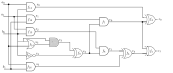
\includegraphics[scale = 0.65]{mas_c}
	\end{center}
	\vspace{-2ex}
	\caption{A 2-bit finite field multiplier}
	\label{mas_c}
	\vspace{-1ex}
\end{figure*}

\begin{Example}
Consider an implementation of a 2-bit finite field multiplier  as shown
in~\autoref{mas_c}. The system is modeled over the ring
$R=\F_4[a_0,b_0,a_1,b_1,s_0,s_1,s_2,s_3,s_4,s_5,e_0,e_1,e_2,e_3,r_0,z_0,$
  $z_1,Z,A,B]$. The multiplier specification is given as $f: Z +
A\cdot B$, and our setup is as follows:
\begin{enumerate}
    \item{Field construction: $\F_4 = \F_2[X]$ (mod $\mathcal{P}$); where $\mathcal{P} = X^2 + X + 1$ is the primitive polynomial used.}
    \item{$Z = z_0 +\al z_1; A = a_0 +\al a_1; B = b_0 +\al b_1;$ are the word level polynomials, and $\al$ is the root of primitive polynomial s.t. $\mathcal{P}(\al)=0$.}
\end{enumerate}
Based on the circuit topology, RTTO$>$ with variable order:
$\{Z\}>\{A>B\}>\{z_0>z_1\}>\{r_0\}>\{e_0>e_1\}>\{e_2\}>\{e_3\}>\{s_0>s_1>s_2>s_3>s_4>s_5\}>\{a_0>a_1>b_0>b_1\}$\\ 
Let $F$ be the set of all polynomials implementing the circuit which is given as:
% \begin{equation*}
% \begin{split}
% f_1:s_0 + a_0*b_0;  &  f_5:r_0 + s_1 + s_2; & f_8:A + a_0 + a_1*\al; \\
% f_2:s_3 + \mathcal{F}(a_1,b_1);  &  f_6:z_0 + s_0 + s_3; & f_9:B + b_0 + b_1*\al;\\
% f_3:s_2 + a_1*b_0;  &  f_7:z_1 + r_0 + s_3; & f_{10}:Z + z_0 + z_1*\al;\\
% f_4:s_1 + a_0*b_1;
% \end{split}
% \begin{equation}
{\small\begin{flalign*}
f_1:Z + z_0 +\al z_1;  &\quad f_9:e_2 + e_3 + s_4;   \\
f_2:A + a_0 +\al a_1;  &\quad f_{10}:e_3 + b_0 + s_3; \\
f_3:B + b_0 +\al b_1;  &\quad f_{11}:s_0 + a_0b_0; \\
f_4:z_0 + s_0 + e_0;	&\quad f_{12}:s_1 + a_1b_1; \\
f_5:z_1 + e_0 + r_0;	&\quad f_{13}:s_2 + a_1b_0; \\
f_6:r_0 + e_1 + s_5;	&\quad f_{14}:s_3 + a_0 + b_0 + a_0b_0; \\
f_7:e_0 + s_1e_2;       &\quad f_{15}:s_4 + b_0 + 1;\\
f_8:e_1 + s_2e_2;		&\quad f_{16}:s_5 + a_0b_1;\\
\end{flalign*}}

Let $J_0 = \langle x_l^4 - x_l\rangle$ denote the ideal of vanishing
polynomials in $R$. 
%% We shall add the ideal of vanishing polynomials $J_0$ for primary inputs.  
%% {\small\begin{flalign*}
%% f_{17}:a_0^2 + a_0; \\
%% f_{18}:a_1^2 + a_1; \\
%% f_{19}:b_0^2 + b_0; \\
%% f_{20}:b_1^2 + b_1; 
%% \end{flalign*}}%
\begin{small}
Then $F = \{f_1,\dots,f_{16}\}, J = \langle F\rangle = \langle
f_1,\dots,f_{16}\rangle$
%J_0 = \langle f_{17},\dots,f_{20}\rangle$
\end{small}
% Due to RTTO$>$, the set of polynomials ($J+J_0$) is in itself a \Grobner basis.\\

For a correct implementation, the specification $f$ is in $J + J_0$.
%vanishes on circuit implementation~(\autoref{lem:imt}):

% \begin{equation}
$f \in \langle f_1,f_2,f_3,\dots,f_{16}\rangle+J_0$

$f \xrightarrow[]{GB(f_1\dots f_{16}, x_l^4-x_l)}_0$

% \end{equation}
% h_4f_4 \in \langle f,f_1,f_2,f_3,f_5,f_6,f_7\rangle\\
% h_4f_4 = f+h_1f_1+h_2f_2+h_3f_3+h_5f_5+h_6f_6+h_7f_7
Now, let us assume the marked gate $f_{10}$ is the \textit{unknown
  component} in the design which is of the form $f_{10} = e_3 + P$,
where $P$ is the unknown function to be implemented by the gate. We
know that under RTTO $>$, the given set of circuit polynomials $F$
itself form a $GB$. Hence to compute $r$, we start reducing the 
specification polynomial $f$ using polynomials from $\langle J + J_0\rangle$.  

We will use the following notations for reduction: '[]' to represent quotient-$h_j$'s, '()' to represent divisor-$f_j$'s, and '\{\}' to represent the partial remainder of every reduction step-$fp_j$'s.

\begin{tiny}
% \begin{split}
$f\xrightarrow[]{f_{1}}[1](Z + z_0 +\al z_1)+\underbrace{{\scriptstyle \{AB+z_0+\al z_1\}}}_\text{$fp_1$}$

$fp_1\xrightarrow[]{f_2}[B](A+a_0+\al a_1)+\underbrace{{\scriptstyle \{Ba_0+\al Ba_1+z_0+\al z_1\}}}_\text{$fp_2$}$

$fp_2\xrightarrow[]{f_3}[a_0+\al a_1](B+b_0+\al b_1)+\underbrace{{\scriptstyle\{z_0+\al z_1+\al a_0b_1+a_0b_0+ (\al+1)a_1b_1 + \al a_1b_0\}}}_\text{$fp_3$}$

$fp_3\xrightarrow[]{f_4}[1](z_0+e_0+s_0)+\underbrace{{\scriptstyle\{\al z_1+e_0+s_0+\al a_0b_1+a_0b_0+(\al+1)a_1b_1+\al a_1b_0\}}}_\text{$fp_4$}$

$fp_4\xrightarrow[]{f_5}[\al](z_1+r_0+e_0)+\underbrace{{\scriptstyle\{\al z_1+e_0+s_0+\al a_0b_1+a_0b_0+(\al+1)a_1b_1+\al a_1b_0\}}}_\text{$fp_5$}$

$fp_5\xrightarrow[]{f_6}[\al](r_0+e_1+s_5)+\underbrace{{\scriptstyle\{(\al+1)e_0+\al e_1+s_0+\al s_5+\al a_0b_1+a_0b_0+(\al+1)a_1b_1+\al a_1b_0\}}}_\text{$fp_6$}$

$fp_6\xrightarrow[]{f_7}[\al+1](e_0+e_2*s_1)+\underbrace{{\scriptstyle\{\al e_1+(\al+1)e_2s_1+s_0+\al s_5+\al a_0b_1+a_0b_0+(\al+1)a_1b_1+\al a_1b_0\}}}_\text{$fp_7$}$

$fp_7\xrightarrow[]{f_8}[\al](e_1+e_2*s_2)+\underbrace{{\scriptstyle\{(\al+1)e_2s_1+\al e_2s_2 + s_0+\al s_5+\al a_0b_1+a_0b_0+(\al+1)a_1b_1+\al a_1b_0\}}}_\text{$fp_8$}$

$fp_8\xrightarrow[]{f_9}[(\al+1)s_1 + \al s_2](e_2+e_3+s_4)+\underbrace{{\scriptstyle\{(\al+1)e_3s_1+ \al e_3s_2 +s_0+(\al+1)s_1s_4+\al s_2s_4+\al s_5+\al a_0b_1+a_0b_0+(\al+1)a_1b_1+\al a_1b_0\}}}_\text{$fp_9$}$
\end{tiny}

\begin{small}

${\scriptstyle fp_9}\xrightarrow[]{{\scriptstyle lt(f_{10})}}[\underbrace{{\scriptstyle (\al+1)s_1+\al s_2}}_\text{$h_{10}$}]({\scriptstyle e_3})+$ 

$\underbrace{{\scriptstyle \{s_0+(\al+1)s_1s_4+\al s_2s_4+\al s_5+\al a_0b_1+a_0b_0+(\al+1)a_1b_1+\al a_1b_0\}}}_\text{$r$}$ 
\end{small}
% \end{split}

Reduction order for $f:$

$f\xrightarrow[]{f_{1}}\xrightarrow[]{f_2}\xrightarrow[]{f_3}\xrightarrow[]{f_4}\xrightarrow[]{f_5}\xrightarrow[]{f_6}\xrightarrow[]{f_7}\xrightarrow[]{f_8}\xrightarrow[]{f_9}\xrightarrow[]{lt(f_{10})}r$

% \begin{equation}
% \begin{split}
% h_4f_4+h_1f_1+h_2f_2+h_3f_3 = f+h_5f_5+h_6f_6+h_7f_7;\\
% h_4(d_0+P(e_1,c))+h_1f_1+h_2f_2+h_3f_3 = f+h_5f_5+h_6f_6+h_7f_7;\\
% h_4*d_0+h_4*P(e_1,c)+h_1f_1+h_2f_2+h_3f_3 = f+h_5f_5+h_6f_6+h_7f_7;\\
% h_4*P(e_1,c)+h_1f_1+h_2f_2+h_3f_3 = h_4*d_0+f+h_5f_5+h_6f_6+h_7f_7;\\
% h_4*P(e_1,c)+h_1f_1+h_2f_2+h_3f_3 = e_0*e_2+a*c+a+b*c+b+c;\\
% h_4*P(e_1,c)+h_1f_1+h_2f_2+h_3f_3 = e_0*e_2+a*c+a+b*c+b+c;
% \end{split}
% \end{equation}
Given: $r,h_{10},f_{11},f_{12},f_{13},f_{14},f_{15},f_{16},J_0$, the
problem can be formulated as an ideal membership test
using \eqref{eqn3} such that: 
\begin{center}
$r \in \langle h_{10},f_{11},f_{12},f_{13},f_{14},f_{15},f_{16}\rangle + \langle J_0\rangle$
\end{center}

The above ideal membership can be solved by expressing $r$ as a
linear combination of the ideal members (~\autoref{lem:imt}). 
\begin{small}
$r = Ph_{10} + h_{11}f_{11} + h_{12}f_{12}+h_{13}f_{13}+h_{14}f_{14}+h_{15}f_{15}+h_{16}f_{16}$ 
\end{small}

In our example, polynomial $r$ can be expressed as
%a linear combination ~(\autoref{lem:imt}) in given member ideal as
%follows:   

% \end{split}
% \end{equation}
\begin{small}
$r = [b_0]h_{10}+[1]f_{11}+[\al+1]f_{12}+[\al s_4 +\al b_0]f_{13}+[0]f_{14}+[(\al+1)s_1+\al a_1b_0]f_{15}+[\al]f_{16}+[0]f_{17}+[0]f_{18}+[0]f_{19}+[0]f_{20}$;
\end{small}

Thus computed $P=b_0$ is a solution to the \textit{unknown component}
$f_{10}$; i.e. $f_{10}: e_3 + b_0$.

Given a solution $P$, we can explore the solution space for 
the gate $f_i$ in terms of variables $x_j$ such that $x_i>x_j$ in the
variable order.
%This can be achieved by computing a quotient of
%ideals~(\autoref{def:quo}) and using different elimination
%ideals~(\autoref{def:elimideal}) with desired variables $x_j$ moved to
%the end of the variable order. 
In our example, $r$ can be written as:
% any linear combination of the ideals:

\begin{align*}
  \begin{split}
    r &= Ph_{10} + h_{11}f_{11} + h_{12}f_{12}+h_{13}f_{13}+h_{14}f_{14}\\
      &\quad +h_{15}f_{15}+h_{16}f_{16}+HJ_0
  \end{split}\\
  \begin{split}
  r & = P'h_{10} + h_{11}'f_{11} +  h_{12}'f_{12}+h_{13}'f_{13}+h_{14}'f_{14}\\
  &\quad +h_{15}'f_{15}+h_{16}'f_{16} + H'J_0
\end{split}
\end{align*}

Re-writing the above two equations:\\
\begin{align}
  \begin{split}
    (P-P')h_{10} &= (h_{11}-h_{11}')f_{11} + (h_{12}-h_{12}')f_{12}\\
    & \quad +\dots+(h_{16}-h_{16}')f_{16}+(H-H')J_0
  \end{split}\\
(P-P')h_{10} & \in  \langle f_{11},f_{12},\dots,f_{16},J_0\rangle\\
(P-P')       &\in     \langle f_{11},f_{12},\dots,f_{16},J_0\rangle:h_{10}\\
(P-P')       & \in  J_Q
\end{align}

The above expression for $J_Q$ represents the quotient of ideals
operation~(\autoref{def:quo}). We can pick any polynomial within
desired variable subset $x_j$ from the result of $J_Q$ and add it to the
computed solution $P$ to arrive at a new solution. 

Under the current $RTTO >$ variable order, the quotient of ideals
operation results in the following polynomials:\\ 
\begin{small}
$g[1]=b_1b_0+b_1+b_0+1\\
g[2]=(\al+1)b_1+(\al+1)*b_1*b_0+(\al+1)*b_0+(\al+1)\\
g[3]=a_1+1\\
g[4]=s_5+a_0b_1\\
g[5]=s_4+b_0+1\\
g[6]=s_3+a_0b_0+a_0+b_0\\
g[7]=s_2+b_0\\
g[8]=s_1+b_1\\
g[9]=s_0+a_0b_0$
\end{small}

Any $P+g[k]$, where $1<k<9$, will work as a solution for the
\textit{unknown component} $f_{10}$. 

Now assume that we know the immediate input variables of the
polynomial $f_{10}$ as $X_{im} = (b_0,s_3)$, we can compute a solution
in terms of these variables by using the elimination
ideal $J_Q \cap \Fq[b_0,s_3]$. The quotient
operation with the elimination ideal results in:\\ 
\begin{small}
$g[1]=s_3b_0 + b_0$
\end{small}

Since, there is only one $g$ from the operation, $P+g[1]=s_3b_0$ also
works as a solution for the \textit{unknown component}: $f_{10}: e_3 +
s_3b_0$. 

\end{Example}

%% \begin{Example}
%% Consider the 2-bit Mastrovito multiplier given in fig.~\ref{mas_c} with variables from ring $\R=\F_2[a_0,b_0$ $,a_1,b_1,s_0,s_1,s_2,s_3,r_0,z_0,z_1,Z,A,B]$. Let us assume $f_2$ to be the unknown gate in the design which is of the form $f_2 = s_3 + P$.\\%\mathcal{F}(a_1,b_1)$.\\


%% % For the given circuit, we define \textit{cuts} across the gates based on heuristics such as dependency and levelization\cite{maciej:2016:1}. A $cut$ is defined as a set of signals that separates primary inputs from primary outputs. The prominence of these cuts is to maintain a variable order across cuts . For example at each cut $cut_m$ from the figure(\ref{tianka_ckt_c}), the following variable set has to be maintained across reductions.
%% % \begin{equation}
%% % \begin{split}
%% % cut_0 = \{a,b,c\} &\quad cut_3= \{z_1,z_2\}\\
%% % cut_1 = \{e_0,e_1,c,e_2\}  &\quad cut_4 = \{z\} \\
%% % cut_2 = \{e_0,d_0,e_2\}
%% % \end{split}
%% % \end{equation}
%% The 2x2 Mastrovito multiplier with specification $f: Z + A\cdot B$, is constructed as follows:
%% % \begin{lalign*}
%% % \begin{split}
%% \begin{enumerate}
%%     \item{Field construction: $\F_4 = \F_2[X]$ (mod $\mathcal{P}$); where $\mathcal{P} = X^2 + X + 1$ is the primitive polynomial used.}
%%     \item{$Z = z_0 + z_1*\al; A = a_0 + a_1*\al; B = b_0 + b_1*\al;$ are the word level polynomials, and $\al$ is the root of primitive polynomial s.t. $\mathcal{P}(\al)=0$.}
%% \end{enumerate}
%% Based on the circuit topology, RTTO$>$ with variable order:
%% $\{Z\}>\{A>B\}>\{z_0>z_1\}>\{r_0>s_0>s_3\}>\{s_1>s_2$ $\}>\{a_0>a_1>b_0>b_1\}$\\ 
%% Let $F$ be the set of all polynomials implementing the circuit which are given as:
%% % \begin{equation*}
%% % \begin{split}
%% % f_1:s_0 + a_0*b_0;  &  f_5:r_0 + s_1 + s_2; & f_8:A + a_0 + a_1*\al; \\
%% % f_2:s_3 + \mathcal{F}(a_1,b_1);  &  f_6:z_0 + s_0 + s_3; & f_9:B + b_0 + b_1*\al;\\
%% % f_3:s_2 + a_1*b_0;  &  f_7:z_1 + r_0 + s_3; & f_{10}:Z + z_0 + z_1*\al;\\
%% % f_4:s_1 + a_0*b_1;
%% % \end{split}
%% % \begin{equation}
%% {\small\begin{flalign*}
%% f_1:s_0 + a_0*b_0;  &\quad  f_5:r_0 + s_1 + s_2; & f_8:A + a_0 + a_1*\al;\\
%% % f_2:s_3 + \mathcal{F}(a_1,b_1);  &\quad  f_6:z_0 + s_0 + s_3; & f_9:B + b_0 + b_1*\al;\\
%% f_2:s_3 + P;  &\quad  f_6:z_0 + s_0 + s_3; & f_9:B + b_0 + b_1*\al;\\
%% f_3:s_2 + a_1*b_0;  &\quad  f_7:z_1 + r_0 + s_3; & f_{10}:Z + z_0 + z_1*\al;\\
%% f_4:s_1 + a_0*b_1;
%% \end{flalign*}}%
%% We shall add the ideal of vanishing polynomials $J_0$ for primary inputs, outputs, and intermediate variables.  
%% {\small\begin{flalign*}
%% f_{11}:a_0^2 + a_0; &\quad f_{15}:s_0^2 + s_0;\quad f_{19}:r_0^2 + r_0;\quad f_{23}:A^4 + A;\\
%% f_{12}:a_1^2 + a_1; &\quad f_{16}:s_1^2 + s_1;\quad f_{20}:z_0^2 + z_0;\quad f_{24}:B^4 + B;\\
%% f_{13}:b_0^2 + b_0; &\quad f_{17}:s_2^2 + s_2;\quad f_{21}:z_1^2 + z_1;\\
%% f_{14}:b_1^2 + b_1; &\quad f_{18}:s_3^2 + s_3;\quad f_{22}:Z^4 + Z;
%% \end{flalign*}}%
%% \begin{small}
%% $F = \{f_1,\dots,f_{10}\}; J = \langle F\rangle = \langle f_1,\dots,f_{10}\rangle; J_0 = \langle f_{11},\dots,f_{24}\rangle$
%% \end{small}
%% % Due to RTTO$>$, the set of polynomials ($J+J_0$) is in itself a \Grobner basis.\\

%% For a correct implementation, specification $f$ vanishes on circuit implementation:
%% % \begin{equation}
%% $f \in \langle f_1,f_2,f_3,\dots,f_{10}\rangle+\langle f_{11},f_{12}$ $,\dots,f_{24}\rangle$,
%% % \end{equation}
%%  where tail of $f_2$ is unknown.
%% % h_4f_4 \in \langle f,f_1,f_2,f_3,f_5,f_6,f_7\rangle\\
%% % h_4f_4 = f+h_1f_1+h_2f_2+h_3f_3+h_5f_5+h_6f_6+h_7f_7

%% We know that under RTTO$>$, the given set of circuit polynomials in itself form a $GB$. Hence to compute $g$, we start reducing the specification polynomial $f$ using polynomials from the set $\langle J + J_0\rangle$. We will use the following notations for reduction: '[]' to represent quotient-$h_i$'s, '()' to represent divisor-$f_i$'s, and '\{\}' to represent the partial remainder of every reduction step-$fp_i$'s.

%% \begin{small}
%% % \begin{split}
%% $f\xrightarrow[]{f_{10}}[1](Z + z_0 + z_1*\al)+\{ A*B+z_0+\al*z_1\}\rightarrow fp_1$

%% $fp_1\xrightarrow[]{f_8}[B](A+a_0+\al*a_1)+\{B*a_0+\al*B*a_1+z_0+\al*z_1\}\rightarrow fp_2$

%% $fp_2\xrightarrow[]{f_9}[a_0+\al*a_1](B+b_0+\al*b_1)+\{z_0+\al*z_1+a_0*b_0+\al*a_0*b_1+\al*a_1*b_0+(\al+1)*a_1*b_1\}\rightarrow fp_3$

%% $fp_3\xrightarrow[]{f_6}[z_0+s_0+s_3](1)+\{\al*z_1+s_0+s_3+a_0*b_0+\al*a_0*b_1+\al*a_1*b_0+(\al+1)*a_1*b_1\}\rightarrow fp_4$

%% $fp_4\xrightarrow[]{f_7}[z_1+r_0+s_3](\al)+\{\al*r_0+s_0+(\al+1)*s_3+a_0*b_0+\al*a_0*b_1+\al*a_1*b_0+(\al+1)*a_1*b_1\}\rightarrow fp_5$

%% $fp_5\xrightarrow[]{f_5}[r_0+s_1+s_2](\al)+\{s_0+(\al+1)*s_3+\al*s_1+\al*s_2+a_0*b_0+\al*a_0*b_1+\al*a_1*b_0+(\al+1)*a_1*b_1\}\rightarrow fp_6$

%% $fp_6\xrightarrow[]{f_1}[s_0+a_0*b_0](1)+\{(\al+1)*s_3+\al*s_1+\al*s_2+\al*a_0*b_1+\al*a_1*b_0+(\al+1)*a_1*b_1\}\rightarrow fp_7$

%% % $fp_6\quad\xrightarrow[]{lt(f_2)}[s_3](\underbrace{x+1}_\text{$h_2$})+\{\underbrace{(x)*s_1+(x)*s_2+(x)*a_0*b_1+(x)*a_1*b_0+(x+1)*a_1*b_1}_\text{$g$}\}$
%% ${\scriptstyle fp_7}\xrightarrow[]{{\scriptstyle lt(f_2)}}[{\scriptstyle s_3}](\underbrace{{\scriptstyle \al+1}}_\text{$h_2$})+\{\underbrace{{\scriptstyle\al s_1+\al s_2+\al a_0b_1+\al a_1b_0+(\al+1)a_1b_1}}_\text{$g$}\}$


%% % \end{split}
%% \end{small}
%% Reduction order for $f:$
%% $f\xrightarrow[]{f_{10}}\xrightarrow[]{f_8}\xrightarrow[]{f_9}\xrightarrow[]{f_6}\xrightarrow[]{f_7}\xrightarrow[]{f_5}\xrightarrow[]{f_1}\xrightarrow[]{lt(f_2)}g$

%% % \begin{equation}
%% % \begin{split}
%% % h_4f_4+h_1f_1+h_2f_2+h_3f_3 = f+h_5f_5+h_6f_6+h_7f_7;\\
%% % h_4(d_0+P(e_1,c))+h_1f_1+h_2f_2+h_3f_3 = f+h_5f_5+h_6f_6+h_7f_7;\\
%% % h_4*d_0+h_4*P(e_1,c)+h_1f_1+h_2f_2+h_3f_3 = f+h_5f_5+h_6f_6+h_7f_7;\\
%% % h_4*P(e_1,c)+h_1f_1+h_2f_2+h_3f_3 = h_4*d_0+f+h_5f_5+h_6f_6+h_7f_7;\\
%% % h_4*P(e_1,c)+h_1f_1+h_2f_2+h_3f_3 = e_0*e_2+a*c+a+b*c+b+c;\\
%% % h_4*P(e_1,c)+h_1f_1+h_2f_2+h_3f_3 = e_0*e_2+a*c+a+b*c+b+c;
%% % \end{split}
%% % \end{equation}
%% Since, we know $g,h_2,f_3,f_4,J_0$, we can formulate it as ideal membership testing problem using~\eqref{member}:
%% \begin{center}
%% $g \in \langle h_2,f_3,f_4\rangle + \langle J_0\rangle$
%% \end{center}

%% This ideal membership test can be done using $lift$ procedure in SINGULAR~\cite{DGPS_410}. The procedure takes polynomial $f$, and ideal $J$ in row matrix form($[J+J_0]$) as inputs, and returns a column matrix $[U]$ as output such that:
%% \begin{small}
%% $f = [U]\cdot [J+J_0]$
%% \end{small}

%% % \begin{equation}
%% % \begin{split}
%% \begin{small}
%% $g = \begin{bmatrix} h_2^{'} & h_3^{'} & \dots & H \end{bmatrix} \cdot 
%%     \begin{bmatrix} h_2 \\ f_3 \\ \vdots \\ x_n^2 + x_n \end{bmatrix}$
%% \end{small}

%% The matrix output can be written in a linear combination as follows: 
%% % \end{split}
%% % \end{equation}
%% \begin{small}
%% $\al*s_1+\al*s_2+\al*a_0*b_1+\al*a_1*b_0+(\al+1)*a_1*b_1 = [\al*s_1+\al*s_2+\al*a_0*b_1+\al*a_1*b_0+(\al+1)*a_1*b_1](\al+1) + [0](s_2 + a_1*b_0) + [0](s_1 + a_0*b_1) + \dots + [0](x_n^2 + x_n)$;
%% \end{small}

%% The $lift$ procedure uses $GB$ to compute the linear combination. Since the generator set has a constant polynomial($\al+1$), the procedure considers it as constant one during membership computation. Hence the output in this case will be a 1x1 matrix with $g$ itself projected as the solution. To normalize the ignored constant, we need to divide(multiply the inverse) the solution $g$ by the constant$(\al+1)$ and reduce it with polynomials \{$f_3,f_4$\} in order to arrive at a implementable solution.

%% \begin{small}
%% $(\al+1)^{-1} = \al$

%% $h_2^{''} = \al*h_2^{'} = \al*(\al*s_1+\al*s_2+\al*a_0*b_1+\al*a_1*b_0+(\al+1)*a_1*b_1)$

%% $h_2^{''} = (\al+1)*s_1+(\al+1)*s_2+(\al+1)*a_0*b_1+(\al+1)*a_1*b_0+ a_1*b_1$

%% $h_2^{''}\xrightarrow[]{f_{3}}\xrightarrow[]{f_4}\underbrace{a_1*b_1}_\text{P}$
%% \end{small}

%% This computed $P$ is a valid solution and can be used as tail of $f_2$. If the resulting $P$ were not a solution in immediate support variables of $s_3$($a_1,b_1$), we could have arrived at this desired solution by devising a new term order. The new term order will have variables $(s_3,a_1,b_1)$ moved to the end on the variable order. We could then compute a $GB$ using the modified term order with the intermediate solution $P$ added as tail of $f_2$. This $GB$ will have one and only one polynomial which is of the form $s_3 + \mathcal{F}(a_1,b_1)$, where $\mathcal{F}$ is the function implemented by the gate for these variables.\\
%% Modified term order $\{Z\}>\{A>B\}>\{z_0>z_1\}>\{r_0>s_0\}>\{s_1>s_2$ $\}>\{a_0>b_0>s_3>a_1>b_1\}$.\\
%% To illustrate the computation of multiple solutions, let's take the current solution $a_1*b_1$ as our $P$. With RTTO$>$ as our term order, from~\eqref{quotcomp}:

%% $a_1*b_1 - P^{'} \in \{f_3,f_4,x_l^q-x_l\}:h_2$;\\
%% The result from quotient of ideal operation is given as:
%% {\small\begin{flalign*}
%% f_3:s_2 + a_1*b_0;  f_{13}:b_0^2 + b_0; f_{23}:A^4 + A;\\
%% f_4:s_1 + a_0*b_1;  f_{14}:b_1^2 + b_1; f_{24}:B^4 + B; \\
%% f_{11}:a_0^2 + a_0; f_{16}:s_1^2 + s_1; \\
%% f_{12}:a_1^2 + a_1; f_{17}:s_2^2 + s_2;
%% \end{flalign*}}%
%% Any polynomial from the above list when added in tail of $f_2$ along with $P$ satisfies the solution set for the given unknown component.
%% \end{Example}

\subsection{Circuit implementation as reference}
Consider a circuit implementation $C$, modeled as polynomials $F = \{f_1,\dots,f_s\}\in \mathbb{F}_q[in_j,x_1,\dots, x_n]$, with $J_1=\langle F \rangle$, $in_j$ as the set of all primary inputs, and $x_n$ as the word level output. Let us assume $f_i:1\le i \le s$ to be the unknown component which is of the special form:
\begin{gather*} 
f_i = x_i + P
\end{gather*}

Let us consider a different circuit $C_1$ as the golden specification which implements the same function as $C$. The reference circuit is modeled as polynomials $D = \{d_1,\dots d_r\}\in \mathbb{F}_q[in_j,y_1,\dots, y_m]$, with $J_2=\langle D \rangle$, $in_j$ as the set of all primary inputs, and $y_m$ as the word level output.

To formulate the problem, we will derive a new circuit structure using the above two implementations ($C,C_1$). Primary input set $in_j$ will be used as the common set of inputs for both the circuits. A new specification polynomial $f$ is derived using the word level outputs as:
\begin{gather}
f_{spec} : (x_n-y_m)
\end{gather}

Now, for a correct implementation, specification $f$ should vanish on the variety of ideal generated by the circuit polynomials i.e., $f$ will be in the ideal generated by the circuit:

$f \in J_1 + J_2 + J_0$: where $J_0$ is the set of all vanishing polynomials from circuits $C$ and $C_1$.

{\small $f \in \langle f_1,\dots,f_s\rangle + \langle d_1,\dots,d_r\rangle + \langle x_l^q-x_l\rangle + \langle y_u^q-y_u\rangle$; $1\le l \le n,1\le u \le m$}

The problem formulation is now exactly same as~\eqref{eqn1} with $f_i$ from circuit $C$ as the unknown gate. Now, we will follow the same procedure as in the first notion to realize the function of the unknown component. Once a solution has been computed, we can verify the circuit using principles from weak $\it{Nullstellensatz}$ by checking if $GB(J_1+J_2+J_0)=\{1\}$.

% \begin{algorithm}
% \caption{Resolve the unknown component for a given circuit}
% \label{algo:unknownComponent}
% \begin{algorithmic}[1]

% \Procedure{$multi\_variate\_division$}{$F,f$}

% \Procedure{$forward\_lifting$}{}

% \EndProcedure
% \end{algorithmic}
% \end{algorithm}

% Thus, $P(u_1)=P(e_1,c)=c$, which can implemented as a simple AND gate with $c$ as both inputs. 

% \begin{figure}[ht]
% 	\begin{center}
% 	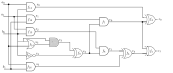
\includegraphics[scale = 0.40]{mas_c}
% 	\end{center}
% 	\vspace{-1ex}
% 	\caption{correct implementation mastrovito}
% 	\label{mas_c}
% 	\vspace{-1ex}
% \end{figure}

% \begin{figure}[ht]
% 	\begin{center}
% 	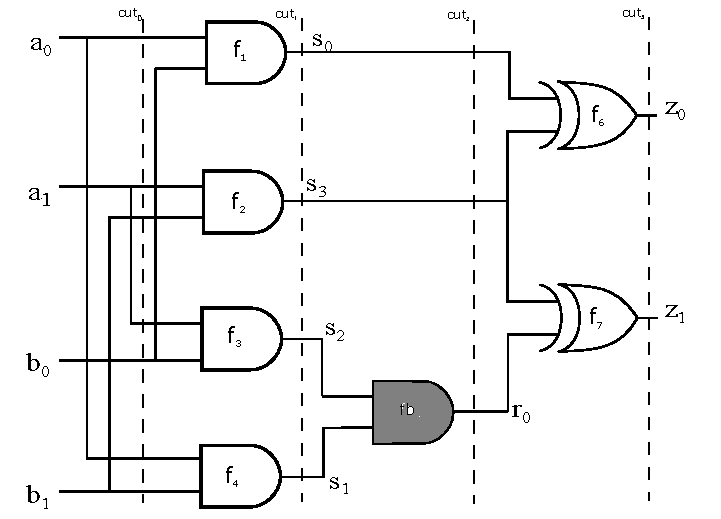
\includegraphics[scale = 0.40]{mas_b}
% 	\end{center}
% 	\vspace{-4ex}
% 	\caption{buggy implementation mastrovito}
% 	\label{mas_b}
% 	\vspace{-2ex}
% \end{figure}

\section{Experiments}
\label{sec:exp}

This section presents experimental results using our approach to debug
the circuits and perform a single-fix rectification. 
We compare results of our implementation against the incremental SAT-based approach presented in~\cite{fujita:2015} wherever it's relevant.
The approach presented in~\cite{fujita:2015} is implemented using PICOSAT~\cite{picosat}. The experiments were performed on a 3.5GHz 
Intel(R) $\text{Core}^{\text{TM}}$ i7-4770K Quad-Core CPU with 32 GB of RAM. The data-path sizes {$k$} are selected according to cryptography standards recommended by U.S. National Institute of Standards and Technology (NIST). 
% In our experiments, the labels $NO$, $NM$, and $NI$ denote 
% % the location of unknown component within the circuit topology. Here $NI$, $NM$, and $NO$ 
% that the unknown component is near the input, middle, and near the output, respectively.
We have performed experiments for the cases when the bugs  are present near 
the input, middle, or near the output of the circuit, represented
using labels $NI$, $NM$, and $NO$ respectively in the tables. All the algorithms
were implemented in SINGULAR~\cite{DGPS}. 

%\subsection{Word level specification v/s Gate level implementation}

\subsubsection{Verification between a word level specification v/s Mastrovito implementation}
~\autoref{masvsspec} presents the results of our approach when the bugs are placed
in a Mastrovito multiplier implementation compared against a specification, which is given in terms of a word level polynomial $f$. 
A Mastrovito multiplier has word level specification $Z = A\times B \pmod{ P(x)}$, 
where $P(x)$ is a given primitive polynomial for the datapath size $k$. The product $A \times B$ 
is computed using an array multiplier architecture, and then the result is reduced modulo $P(x)$. 
Bugs in the circuit are introduced, and the presence of the bugs is
detetced. Then we apply our approach to check for single-fix
rectification interatively on the nets selected in $\mathcal{N}$. If
rectification is feasible at $x_i$, the unknown component problem is
solved to identify a rectification function. 

%% The circuit implementation is modeled as a set of polynomials $F=\{f_1,\dots f_i,\dots,f_s\}$. The 
%% approach then follows the partial reduction of specification polynomial $f$ until leading term of $f_i$ while
%% recording the intermediate quotients and remainders. We then represent the partial remainder as a linear combination
%% using the remaining gate polynomials and the quotient to obtain the solution $P$.
We 
are able to verify and debug the circuits for upto 64-bits within our
stipulated Time Out ($TO$)  period.

\begin{table*}[hbt]
\centering
\caption{{\small Single fix rectification debug in Mastrovito circuit against word level specification}. Time is in seconds; $k$ = Datapath Size, \#Gates = No. of gates, K = $10^3$, \textit{a}=verification time, \textit{b}=time for rectification check, \textit{c}=time for component correction computation,\textit{d}=total time}
\label{masvsspec}
\begin{tabular}{| c | c | c | c | c | c | c | c | c | c | c | c | c | c |} \hline
\multirow{3}{*}{\textbf{k}}& \multirow{3}{*}{\#Gates} & \multicolumn{12}{ c |}{Our implementation}\\ \cline{3-14}
&&\multicolumn{4}{ c |}{\it NI}&\multicolumn{4}{ c |}{\it NM}&\multicolumn{4}{ c |}{\it NO}\\ \hline
&&{\it a}&{\it b}&{\it c} &{\it d}&{\it a}&{\it b}&{\it c} &{\it d}&{\it a}&{\it b}&{\it c} &{\it d}\\ \hline
9 & 0.23K & 0.0 & 0.0 & 0.0 & 0.0 & 0.0 & 0.0 & 0.0 & 0.0 & 0.0 & 0.0 & 0.0  & 0.0\\ \hline
10& 0.29K & 0.0 & 0.0 & 0.0 & 0.0 & 0.0 & 0.0 & 0.0 & 0.0 & 0.0 & 0.0 & 0.0  & 0.0\\ \hline
11& 0.35K & 0.0 & 0.0 & 0.1 & 0.1 & 0.0 & 0.0 & 0.1 & 0.1 & 0.0 & 0.0 & 0.1  & 0.1\\ \hline
12& 0.97K & 0.1 & 0.5 & 0.4 & 0.9 & 0.2 & 0.5 & 0.4 & 1.1 & 0.5 & 0.8 & 0.4  & 1.7\\ \hline
13& 0.82K & 0.1 & 0.3 & 0.2 & 0.6 & 0.2 & 0.6 & 0.2 & 1.0 & 0.7 & 0.8 & 0.2  & 1.7\\ \hline
16& 1.8K  & 0.9 & 2.6 & 1.0 & 4.5 & 1.1 & 3.5 & 1.0 & 5.6 & 2.8 & 5.3 & 1.0  & 9.1\\ \hline
32& 5.4K  & 36  & 110 & 42  & 188 & 40  & 160 & 47  & 247 & 38  & 240 & 150  & 428\\ \hline
64& 21.8K & 2210& 7100 & 2432 & 9532 & 2200 & 8000 & 2575 & 12775 & 2150& 7840 & 10020 & 20010 \\ \hline
\end{tabular}
\end{table*}


\begin{table*}[hbt]
\centering
\caption{{\small Rectification for Mastrovito circuit with Montgomery circuit as specification}. Time is in seconds; $k$ = Datapath Size, \#Gates = No. of gates, (TO): Time-Out = 3 hrs, K = $10^3$,\textit{a}=verification time, \textit{b}=time for rectification check, \textit{c}=time for component correction computation, \textit{d}=total time}
\label{masusmontspec}
\begin{tabular}{| c | c |  c | c | c | c | c | c | c | c | c | c | c | c | c | c | c |} \hline
\multirow{4}{*}{\textbf{k}}& \multirow{4}{*}{\#Gates} & \multicolumn{3}{ c |}{Incremental SAT\textbf{~\cite{fujita:2015}}}& \multicolumn{12}{ c |}{Our Approach}\\ \cline{3-17}
&&\multirow{2}{*}{\it NI}&\multirow{2}{*}{\it NM}&\multirow{2}{*}{\it NO}&\multicolumn{4}{ c |}{\it NI}&\multicolumn{4}{ c |}{\it NM}&\multicolumn{4}{ c |}{\it NO} \\ \cline{6-17}
&&&&&{\it a}&{\it b}&{\it c} &{\it d}&{\it a}&{\it b}&{\it c} &{\it d}&{\it a}&{\it b}&{\it c} &{\it d}\\ \hline
9 & 0.6K & 35   & 37   & 33    & 0.1 & 0.5 & 0.2 & 0.8 & 0.2 & 0.2 & 0.1 & 0.5 & 1.8 & 2.2 & 0.6 & 4.6 \\ \hline
10& 0.7K & 231  & 215  & 214   & 0.3 & 1   & 0.5 & 1.8 & 0.3 & 1   & 0.8 & 2.1 & 4.7 & 5.4 & 0.2 & 10 \\ \hline
11& 0.9K & 2090 & 1927 & 2000  & 0.6 & 2   & 1   & 3.6 & 0.8 & 2   & 32  & 35  & 9 & 10 & 0.4 & 19 \\ \hline
12& 1.6K & 8676 & 23400& 24085 & 3.2 & 9.6 & 3.5 & 16  & 3.2 & 9.3 & 12  & 24  & 155 & 160 & 1.6 & 316 \\ \hline
13& 1.7K & TO   & TO   & TO    & 3.3 & 10  & 4.5 & 18  & 3.5 & 10 & 22 & 35 & 170 & 177 & 1.6 & 349 \\ \hline
16& 3K   & TO   & TO   & TO    & 27  & 81  & 35  & 143 & 28 & 83 & 48 & 159 & 210 & 176 & 2.5 & 389\\ \hline
32& 9.8K & TO   & TO   & TO    &  2060   & 6595    & 1870&  10525   & 2100 & 7320 & 1289 & 10709 & 2215 & 7870 & 1204 & 11289 \\ \hline
\end{tabular}
\end{table*}




% \begin{table}[H]
% \centering
% \caption{{Single fix rectification debug in Mastrovito circuit against word level specification}. Time is in seconds; $k$ = Datapath Size, \#Gates = No. of gates, K = $10^3$}
% \label{masvsspec}
% \begin{tabular}{| c | c | c | c | c | c | c | c | c | c | c | c | c | c | c | c | c |} \hline
% \multirow{3}{*}{\textbf{k}}& \#Gates & \multicolumn{15}{ c |}{Our implementation}\\ \cline{3-17}
% &&\multicolumn{5}{ c |}{\it NI}&\multicolumn{5}{ c |}{\it NM}&\multicolumn{5}{ c |}{\it NO}\\ \hline
% &&{\it a}&{\it b}&{\it c} &{\it d}&{\it e}&{\it a}&{\it b}&{\it c} &{\it d}&{\it e}&{\it a}&{\it b}&{\it c} &{\it d}&{\it e}\\ \hline
% 9& 0.23K & 0.0 & 0.1 & 0.0 & 0.2 & 0.0 & 0.1 & 0.0 & 0.2 & 0.0 & 0.2 & 0.0 & 0.3\\ \hline
% 10& 0.29K & 0.0 & 0.3 & 0.0 & 0.3 & 0.0 & 0.3 & 0.0 & 0.3 & 0.0 & 0.4 & 0.0 & 1.4\\ \hline
% 11& 0.35K & 0.0 & 0.2 & 0.0 & 0.3 & 0.0 & 0.3 & 0.0 & 0.4 & 0.0 & 0.6 & 0.0 & 0.7\\ \hline
% 12& 0.97K & 0.1 & 7.5 & 0.5 & 8.0 & 0.2 & 10.1 & 0.5 & 10.5 & 0.5 & 121.2 & 0.8 & 121.3\\ \hline
% 13& 0.82K & 0.1 & 4.3 & 0.3 & 4.5 & 0.2 & 11.3 & 0.6 & 11.2 & 0.7 & 156.3 & 0.8 & 158.1\\ \hline
% 16& 1.8K & 0.9 & 14.1 & 2.6 & 30.2 & 1.1 & 33.1 & 3.5 & 34.9 & 2.8 & 501.2 & 5.3 & 503.0\\ \hline
% 32& 5.4K & 36.8 & 378.6 & 110.5 & 544.7 & 40.0 & 567.1 & 160.3 & 767.2 & 38.1 & 1286.1 & 240.3 & 1342.7\\ \hline
% %64& 21.8K & 36.8 & 378.6 & 110.5 & 544.7 & 40.0 & 567.1 & 160.3 & 767.2 & 38.1 & 1286.1 & 240.3 & 1342.7\\ \hline
% \end{tabular}
% \end{table}

\subsubsection{Word level specification v/s Point addition implementation}
Point addition is an important operation required for the task of encryption, decryption 
and authentication in Elliptic Curve Cryptography (ECC). 
Modern approaches represent the points in projective
coordinate systems, {\it e.g.}, the L$\acute{o}$pez-Dahab (LD) projective coordinate, due to which the point addition 
operation can be implemented as polynomials in the field.

\begin{Example}
{\it\small %Consider point addition in L$\acute{o}$pez-Dahab (LD) projective
  %coordinate.
  Given an elliptic curve: $Y^2 + XYZ = X^3Z + aX^2Z^2 +
  bZ^4$ over $\mathbb{F}_{2^k}$, where $X,Y,Z \in \mathbb{F}_{2^k}$ and similarly, $a, b$ are
  constants from the field. Point addition over the
  elliptic curve is ($X_3$, $Y_3$, $Z_3$) = ($X_1$, $Y_1$, $Z_1$) +
  ($X_2$, $Y_2$, $1$).  Then $X_3$, $Y_3$, $Z_3$ can be computed as
  follows:}
\vspace{-0.09in}
{\tiny
\begin{align*}
&A = Y_2 \cdot Z_1^2 + Y_1  &&B = X_2 \cdot Z_1 + X_1 \\
&C = Z_1 \cdot B  &&D = B^2 \cdot(C + a Z_1^2) \\
&Z_3 = C^2 && E = A \cdot C  \\
&X_3 = A^2 + D + E &&F = X_3 + X_2 \cdot Z_3 \\
&G = X_3 + Y_2\cdot Z_3 && Y_3 = E\cdot F + Z_3 \cdot G
\end{align*}
}
\vspace{-0.38in}

\end{Example}

Each of the polynomials in the above design are implemented as a
(gate-level) logic block and are interconnected to obtain final
outputs $X_3,Y_3$ and $Z_3$. ~\autoref{pdvsspec} shows
the comparison of the time required for debugging and rectification
for the implementation of the block $D= B^2\cdot(C + aZ_1^2)$. 

\begin{table}[H]
\centering
\caption{{\small Single fix rectification debug in Point Addition circuits against word level specification}. Time is in seconds; $k$ = Datapath Size, \#Gates = No. of gates, K = $10^3$, \textit{a}=verification time, \textit{b}=time for rectification check,\textit{c}=time for component correction computation,\textit{d}=total time}
\label{pdvsspec}
\begin{tabular}{| c | c | c | c | c | c | c | c | c | c | c | c | c | c |} \hline
\multirow{3}{*}{\textbf{k}}& \multirow{3}{*}{\#Gates} & \multicolumn{12}{ c |}{Our implementation}\\ \cline{3-14}
&&\multicolumn{4}{ c |}{\it NI}&\multicolumn{4}{ c |}{\it NM}&\multicolumn{4}{ c |}{\it NO}\\ \hline
&&{\it a}&{\it b}&{\it c} &{\it d}&{\it a}&{\it b}&{\it c} &{\it d}&{\it a}&{\it b}&{\it c} &{\it d}\\ \hline
8 & 244  & 0.0 & 0.0 & 0.0 & 0.0 & 0.0 & 0.0 & 0.0 & 0.0 & 0.0 & 0.0 & 0.0 & 0.0\\ \hline
16& 1.2K & 1.3 & 3.9 & 1.5 & 6.7 & 1.2 & 3.7 & 2   & 6.9 & 1.2 & 3.7 & 1.8 & 6.7\\ \hline
32& 3.9K & 37  & 112 & 77  & 226 & 38  & 110 & 22  & 170 & 37  & 108 & 35  & 180\\ \hline
%64& 15K  & 40  & 2283&  &  &  &  &  &  &  &  &   & \\ \hline
\end{tabular}
\end{table}

\subsubsection{Word level specification v/s Barrett reduction implementation}
Barrett reduction
%~\cite{barrett}
is the other widely used multiplier design
method adopted in cryptography system designs. 
Based on Barrett reduction, a multiplier can be designed in two steps:
multiplication $R = A \times B$ and a subsequent Barrett reduction G =
R (mod P). ~\autoref{bartvsspec} shows results for debugging and rectification of
Barrett multipliers against a polynomial specification. 

\begin{table}[H]
\centering
\caption{{\small Single fix rectification debug in Barrett reduction circuits against word level specification}. Time is in seconds; $k$ = Datapath Size, \#Gates = No. of gates, K = $10^3$, \textit{a}=verification time, \textit{b}=time for rectification check,\textit{c}=time for component correction computation,\textit{d}=total time}
\label{bartvsspec}
\begin{tabular}{| c | c | c | c | c | c | c | c | c | c | c | c | c | c |} \hline
\multirow{3}{*}{\textbf{k}}& \multirow{3}{*}{\#Gates} & \multicolumn{12}{ c |}{Our implementation}\\ \cline{3-14}
&&\multicolumn{4}{ c |}{\it NI}&\multicolumn{4}{ c |}{\it NM}&\multicolumn{4}{ c |}{\it NO}\\ \hline
&&{\it a}&{\it b}&{\it c} &{\it d}&{\it a}&{\it b}&{\it c} &{\it d}&{\it a}&{\it b}&{\it c} &{\it d}\\ \hline
8 & 134 & 0.0 & 0.0 & 0.0 & 0.0 & 0.0 & 0.0 & 0.0 & 0.0 & 0.0 & 0.0 & 0.0 & 0.0\\ \hline
16& 427 & 0.1 & 0.0 & 0.0 & 0.1 & 0.0 & 0.2 & 0.1 & 0.3 & 0.0 & 0.1 & 0.3 & 0.4\\ \hline
32& 1.4K & 0.4 & 1.4 & 0.1 & 1.9 & 0.5 & 1.5 & 0.1 & 2.1 & 1.2 & 2.2 & 1.1 & 4.5\\ \hline
64& 4.9K & 19  & 58  & 5.4 & 82  & 21  & 60  & 1.7 & 83  & 63  & 104 & 141 & 308\\ \hline
\end{tabular}
\end{table}

Since the SAT-based approach cannot be applied against a word level specification polynomial, 
we perform experiments while using another multiplier implementation as the specification.

\subsubsection{Verification between a specification and implementation
  given as gate level circuits: Mastrovito v/s Montgomery multipliers}

%% \begin{table*}[ht]
%% \centering
%% \caption{{Resolving Unknown Component in Mastrovito circuit with Montgomery circuit as specification}. Time is in seconds; $k$ = Datapath Size, \#Gates = No. of gates, (TO): Time-Out = 3 hrs, K = $10^3$,\textit{a}=verification time, \textit{b}=time for rectification check,\textit{c}=time for component correction computation,\textit{d}=total time}
%% \label{masusmontspec}
%% \begin{tabular}{| c | c |  c | c | c | c | c | c | c | c | c | c | c | c | c | c | c |} \hline
%% \multirow{4}{*}{\textbf{k}}& \multirow{4}{*}{\#Gates} & \multicolumn{3}{ c |}{Incremental SAT\textbf{~\cite{fujita:2015}}}& \multicolumn{12}{ c |}{Our Approach}\\ \cline{3-17}
%% &&\multirow{2}{*}{\it NI}&\multirow{2}{*}{\it NM}&\multirow{2}{*}{\it NO}&\multicolumn{4}{ c |}{\it NI}&\multicolumn{4}{ c |}{\it NM}&\multicolumn{4}{ c |}{\it NO} \\ \cline{6-17}
%% &&&&&{\it a}&{\it b}&{\it c} &{\it d}&{\it a}&{\it b}&{\it c} &{\it d}&{\it a}&{\it b}&{\it c} &{\it d}\\ \hline
%% 9 & 0.6K & 35   & 37   & 33    & 0.1 & 0.5 & 0.2 & 0.8 & 0.2 & 0.2 & 0.1 & 0.5 & 1.8 & 2.2 & 0.6 & 4.6 \\ \hline
%% 10& 0.7K & 231  & 215  & 214   & 0.3 & 1   & 0.5 & 1.8 & 0.3 & 1   & 0.8 & 2.1 & 4.7 & 5.4 & 0.2 & 10 \\ \hline
%% 11& 0.9K & 2090 & 1927 & 2000  & 0.6 & 2   & 1   & 3.6 & 0.8 & 2   & 32  & 35  & 9 & 10 & 0.4 & 19 \\ \hline
%% 12& 1.6K & 8676 & 23400& 24085 & 3.2 & 9.6 & 3.5 & 16  & 3.2 & 9.3 & 12  & 24  & 155 & 160 & 1.6 & 316 \\ \hline
%% 13& 1.7K & TO   & TO   & TO    & 3.3 & 10  & 4.5 & 18  & 3.5 & 10 & 22 & 35 & 170 & 177 & 1.6 & 349 \\ \hline
%% 16& 3K   & TO   & TO   & TO    & 27  & 81  & 35  & 143 & 28 & 83 & 48 & 159 & 210 & 176 & 2.5 & 389\\ \hline
%% 32& 9.8K & TO   & TO   & TO    &     &     & 1870&     &  &  & 1289 &  &  &  & 1204 &  \\ \hline
%% \end{tabular}
%% \end{table*}

%\subsubsection{Mastrovito v/s Montgomery}
%% \begin{figure}[H]
%%   \centering
%%   %\def\svgwidth{340pt}
%%   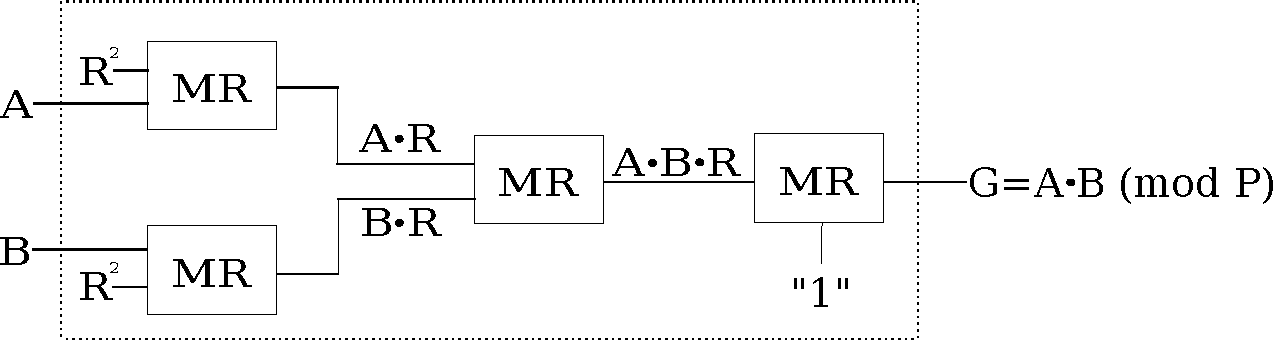
\includegraphics[scale=0.34]{new_mmcircuit-eps-converted-to}
%%   \caption{Montgomery multiplication.}
%%   \label{montfig}
%%   \end{figure}

Montgomery architectures~\cite{acar:1998},~\cite{wu:2002},
% \cite{Barrett:1987} 
~\cite{knezevic:2008} are considered more efficient than Mastrovito multipliers for exponentiation, 
as they do not require explicit reduction modulo $P(x)$ after each step.
%% ~\autoref{montfig} shows the structure of a Montgomery
%% multiplier. Each MR block computes $A\cdot B\cdot R^{-1}$, where $R$
%% is selected as a power of a base ($\alpha^{k}$) and $R^{-1}$ is the multiplicative 
%% inverse of $R$ in $\mathbb{F}_{2^k}$. As this operation cannot compute $A\cdot B$
%% directly, we need to pre-compute $A\cdot R$ and $B\cdot R$ as shown in the~\autoref{montfig}. 
%% We denote the leftmost
%% two blocks as Block A (upper) and B (lower), the middle block as Block
%% C and the output block as Block D.
% We have presented results for GBR
%on both \textit{flattened} and \textit{hierarchical} netlists of these
% multipliers.

~\autoref{masusmontspec} presents the results of our approach to debug
and rectification with the bugs placed in the Montgomery multiplier
with a Mastrovito multiplier circuit used as the specification. While
the approach~\cite{fujita:2015} finds a satisfying transformation
assignment which can be mapped to a library gate, our approach debugs
the circuit and finds a single fix rectification function. As shown in
the table, our approach shows improvement by several orders of
magnitude over \cite{fujita:2015}. 

%The comparison of bug placement reflects the complexity involved in
%debugging circuits where the bug lies in the deeper part ($NO$) of the
%topology.
It takes considerable amount of time for verification and
rectification check when the bug is close to the output. We are
working on further improving the experiments by employing better data
structures like  
ZBDDs~(\cite{minato:zbdd}), and devising better heuristics to perform
rectification check.
%We are also looking into efficient
%implementations for representing the partial remainder as a linear
%combination of an ideal during correction computation.
Due to several limitations w.r.t number of ring variables that can be
declared in SINGULAR, we have had to restrict our experiments within
64-bit data-path size.   

\section{Conclusions}

This paper has presented a fully automated debug approach for single fix rectification under RTTO$>$ based on \Grobner basis reductions and ideal
membership test. We presented a procedure to test for the existence of utilized the duality of varieties and ideals to check for the existence of single fix rectification at a given net. 
The experimental results demonstrate the efficacy of our approach for finite field arithmetic circuits where we achieve several orders of magnitude
improvement as compared to recent SAT-based approach. 
As part of our future work, we are working on improving the efficiency of our implementation to target higher bit-widths. We are also investigating how the current procedure can be extended to cover integer arithmetic circuits.
Further research also includes exploring the current approach for
the case of multi-fix rectification.  

\section{Conclusion and future work}
This paper has presented an approach based on \Grobner basis reductions and ideal
membership test to compute a function implemented by an unknown component in a circuit which models
a given specification. 
% We presented a procedure to systematically use \Grobner basis based reduction and ideal membership testing to arrive at a 
% solution, such that the resulting logic function of the circuit conforms to the reference specification. 
The paper also utilizes the concept of quotient of ideals to derive multiple solutions
for the unknown component. The experimental results demonstrate the efficiency of our approach 
for finite field arithmetic circuits where we achieve several orders of 
magnitude improvement as compared to recent SAT-based approach. 
We also present the theory for exploring the solution for the unknown 
component in terms of its immediate inputs.  
% The most desired solution which is in terms of immediate support 
% variables of the unknown component relies on expensive \Grobner basis re-computation 
% with a different term order. 
% As part of our future work, we are exploring heuristics 
% in order to arrive at a guided, simple implementable solutions set for $P$.
% The current set-up deals with one unknown 
% component or sub-circuit, 
As part of our future work, we are working on extending the current approach  
for the case of multiple independent/dependent bugs in the design along
with identifying the potential locations where the circuit can be rectified 
with the current setup.  
% Also, identifying the bug location, 
% which is the primary concern in the overall scope of automated debugging 
% needs to be addressed as well. 
%%%%%%%%%%%%%%%%%%%% The bibliography %%%%%%%%%%%%%%%%%%%%%%%%%%%%

\bibliographystyle{IEEEtran}
\bibliography{vikas,utkarsh,tim,xiaojun}

\end{document}

%%%%%%%%%%%%%%%%%%%%%%%%%%%  End of IEEEsample.tex  %%%%%%%%%%%%%%%%%%%%%%%%%%%
